\documentclass[twoside,openleft,reqno,a4paper,final]{book}
%%% Remove the next two lines if you want the figures at their place    
%\usepackage[figuresonly,nolists,nomarkers]{endfloat}
%\renewcommand{\processdelayedfloats}{}
\usepackage[T1]{fontenc}
\usepackage[utf8]{inputenc}
\usepackage[version=4]{mhchem}
\usepackage{hyperref,booktabs,algpseudocode,algorithm,booktabs,titlesec,setspace,relsize}
\usepackage{amsmath,xcolor,graphicx,float,subcaption}
\usepackage[toc,page]{appendix}
%\pagenumbering{roman}  http://www.markschenk.com/tensegrity/latexexplanation.html
 %A4 (210 mm x 297 mm)  https://tex.stackexchange.com/questions/20538/what-is-the-right-order-when-using-frontmatter-tableofcontents-mainmatter
%\addtolength{\textwidth}{12mm}%210
%\addtolength{\evensidemargin}{-4mm}
%\addtolength{\oddsidemargin}{-8mm}
%\addtolength{\textheight}{35mm}%297
\setlength{\parskip}{1.3ex plus 0.2ex minus 0.2ex}
\setlength{\parindent}{0pt}

\usepackage[bindingoffset=25mm, left=15mm, right=15mm,top=30mm, bottom=20mm]{geometry}

\usepackage{fancyhdr}
\pagestyle{fancy}
\renewcommand{\chaptermark}[1]{\markboth{\thechapter~-~#1}{}}
 \fancyhf{}
  \fancyhead[LE]{\itshape   \thepage}
 \fancyhead[RE]{\itshape  \nouppercase{\rightmark}} %\nouppercase !
  \fancyhead[LO]{\itshape  \nouppercase{\leftmark }}%thechapter
 \fancyhead[RO]{\itshape  \thepage} %\nouppercase !
%  \cfoot{\thepage}
%\renewcommand{\footrulewidth}{\headrulewidth}
\pagestyle{fancy}

\newcommand{\ch}[1]{\MakeUppercase{\ce{#1}}}  % version 1
\newcommand{\multiref}[2]{\autoref{#1}-\ref{#2}} % from - to
\newcommand{\qfig}[4]{\begin{figure}[H]\centering\includegraphics[width=#4]{#1}\caption{#3}\label{#2}\end{figure}\newpage}
% location,label,caption,width


\usepackage[space=true]{grffile}


\def\blankpage{%
      \clearpage%
      \thispagestyle{empty}%
      \addtocounter{page}{-2}%
      \null%
      \clearpage}




\algnewcommand\algorithmicforeach{\textbf{for each}}
\algdef{S}[FOR]{ForEach}[1]{\algorithmicforeach\ #1\ :}

% dont have & in citations, and clear to fix error



\newcommand{\dfig}[4]{
\newpage
\begin{figure}[H]
\centering\includegraphics[width=.45\textwidth]{#1}
\centering\includegraphics[width=.45\textwidth]{#2}
\caption{ Colouring #4 }
\label{#3}
\end{figure}
\newpage
}


%%%%%%

% location,label,caption,width





\author{Dan Ellis }
\date{March 2019}




\begin{document}
% \newgeometry{oneside}


\titleformat{\paragraph}[hang]{\normalfont\normalsize\bfseries}{\theparagraph}{1em}{}
\titlespacing*{\paragraph}{0pt}{3.25ex plus 1ex minus .2ex}{1em}

\setcounter{secnumdepth}{3}
\setcounter{tocdepth}{5}
%\cleardoublepage
\setcounter{page}{101}
\setcounter{chapter}{10}

% \maketitle
\cleardoublepage{}
\chapter{ What can machines tell us about atmospheric chemistry? }
\cleardoublepage{}
\restoregeometry
\vspace*{0.15\paperheight} 
\begin{center}
\begin{quotation}
  \large{\emph{\textbf{``So, in the interests of survival, they trained themselves to be agreeing machines instead of thinking machines. All their minds had to do was to discover what other people were thinking, and then they thought that, too.''} }  }  \\
  \begin{flushright}
  - Kurt Vonnegut, \textit{Breakfast of Champions} 

  \end{flushright}
 \end{quotation}
\end{center}


%\blankpage
\doublespacing
% \onehalfspacing

\newpage
\setlength{\footnotesep}{0.5cm}
\raggedbottom %group writing to top of page!
%
%  
\section{Introduction}
The node-link (ball-stick) [REF SECTION] style structure has long been used to represent real-world relationships between items. Such a structure is complementary to our cognitive disposition towards pattern recognition [citep]. It is for this reason that the node-link visualisation format has been used for anything ranging from transportation maps [citep BECK] to the differentiation of ancestorial lineages of the human race (\autoref{fig:skulls}). However, the abundance and complexity of real-world data often present us with difficulties in manually representing it in a useful form. In SECTION XX it is suggested this may be overcome with the use of computational analysis and automated visualisation tools. Such methods usually require a level of data manipulation to transform the data into a machine parseable form. 

\begin{figure}[H]
     \centering
         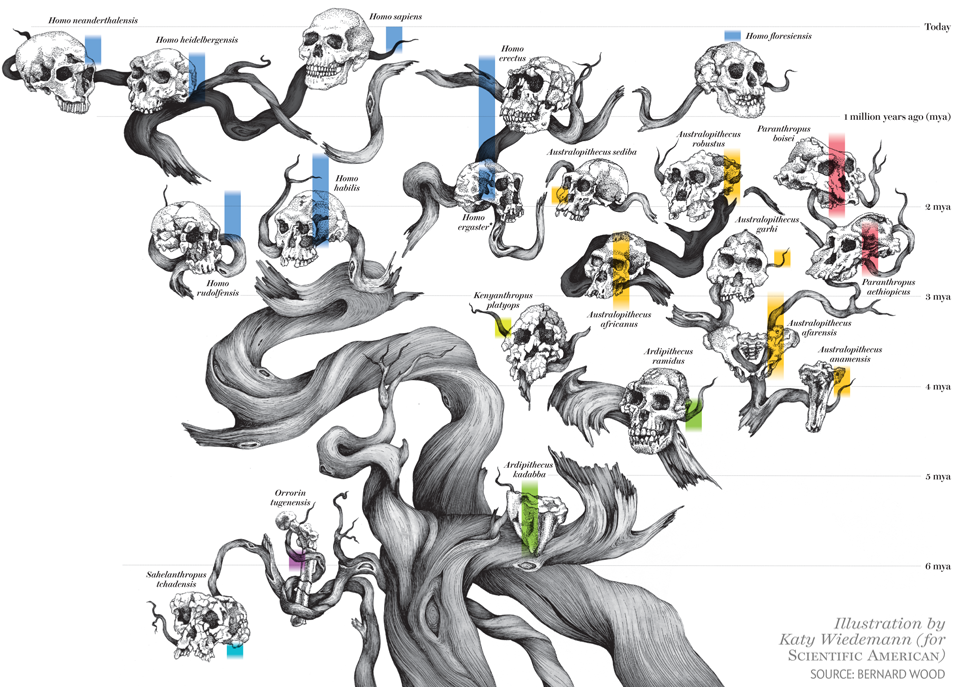
\includegraphics[width=\textwidth]{figures_c3/humanskulls.png}

        \caption[Caption for LOF]{\textbf{The human family tree.} This is a visual depiction of the human lineage, starting with our common ancestorial roots. In SECTION it was shown that the use of trees / graphs\protect\footnotemark is useful in showing relationships between items. Source: \citep{skull}}
        \label{fig:skulls}
\end{figure}
%inserted in the figure caption
\footnotetext{A tree is a special case of a graph}



In the field of mathematics a graph, $G(\nu,\epsilon,\omega)$, is defined as a function of items (vertices\footnote{The term node, item or vertex shall be used interchangeably for the remainder of this chapter. This also applies to links/relationships/edges and edge-weight/strength}), $\nu$ which are connected through a series of connections (or edges$^1$) representing any relationships between them, $\epsilon$. Since relationships in the real world are rarely equivalent, we then encode the importance of each link in the form of an edge weight, or strength - $\omega$. Such formats allow both numerical and computational algorithms to understand and interpret the graph structure, providing us with information about the data or make use of automated layout programs for visualisation. 


This chapter builds on the work shown in SECTION XXX - where 
the ability to represent complex data in the form of a graph was used to (visually) draw information regarding network structure and temporal changes. Here I will begin by exploring situations where the visual representation of many, large or complex networks is impractical. We start by introducing a series of mathematical approaches which are capable of quantifying the graph (and nodes within it) and apply them to the co-author network for papers regarding the Master Chemical Mechanism, \autoref{sec:graphmetrics}. Following these global metrics are used to categorise the chemistry within different mechanism subsets, and provide us with an insight to the chemistry structure (SECT LABEL) and finally apply these to real-world simulations representing a range of environments (marine, rainforest and urban) in SECTREF.


\textit{
This allows for a higher level of automated analysis which can be used to batch process, analyse and categorise chemical simulations. \autoref{sec:graphmetrics} begins by introducing the most common of the graph metrics which can be used for analysis. To do this a citation graph is generated by web-scraping google scholar results. 
}


\section{Graph Metrics}\label{sec:graphmetrics}

An increase in the ability to gather and store data results in a difficulty to understand it (ref SECTION). The production of large, multivariate networks of inexplicable complexity greatly hinders our ability to draw out meaningful conclusions based on visualisation alone. This means that much like the generation of mechanism, or creating semi-automated graph drawing layouts, we must rely on the field of mathematics coupled with computational aid (REF SECTION).

Numerical algorithm, derived from the field of Graph Theory can be used to circumvent the need for individual graph analysis and provide us with information about the network. One such subset of numerical algorithms are regarded as "centrality metrics", and may be used to rank the role and importance (centrality) of a node. In the following sub-section, the most common (REF PAPER) centrality metrics are discussed and applied to the MCM citation network. 


\subsection{Centrality metrics and academic publishing.}


One common application for graph analysis and visualisation is the representation and prediction of citation counts within academic journals \citep{cocite,google,naturecitation,netcoauthor}. Here network-visualisation techniques may be used to highlight the origins of a paper - for instance, \autoref{fig:naturecover} shows the multi-disciplinary research which underpins 6 prominent discoveries in the last 150 years. 

To the properties presented by different centrality metrics (described above), we apply them to an approximate representation of the citation graph relating to the Master Chemical Mechanism (\autoref{sec:metricmcm}).



\subsection{The Master Chemical Mechanism (MCM)}\label{sec:metricmcm}

The MCM, \citep{mcm}, is a near explicit representation of our foremost understanding of gas-phase tropospheric chemistry. The mechanism describes the oxidation of 143 primary emitted VOCs and the respective rates at which this occurs. It has been used in the... 



 Information on the chemistry, - x species - y ... first published and how this can be used with regards to the following algorithms are presented in REF JENKINS 15 ACP. 


\begin{figure}[H]
     \centering
         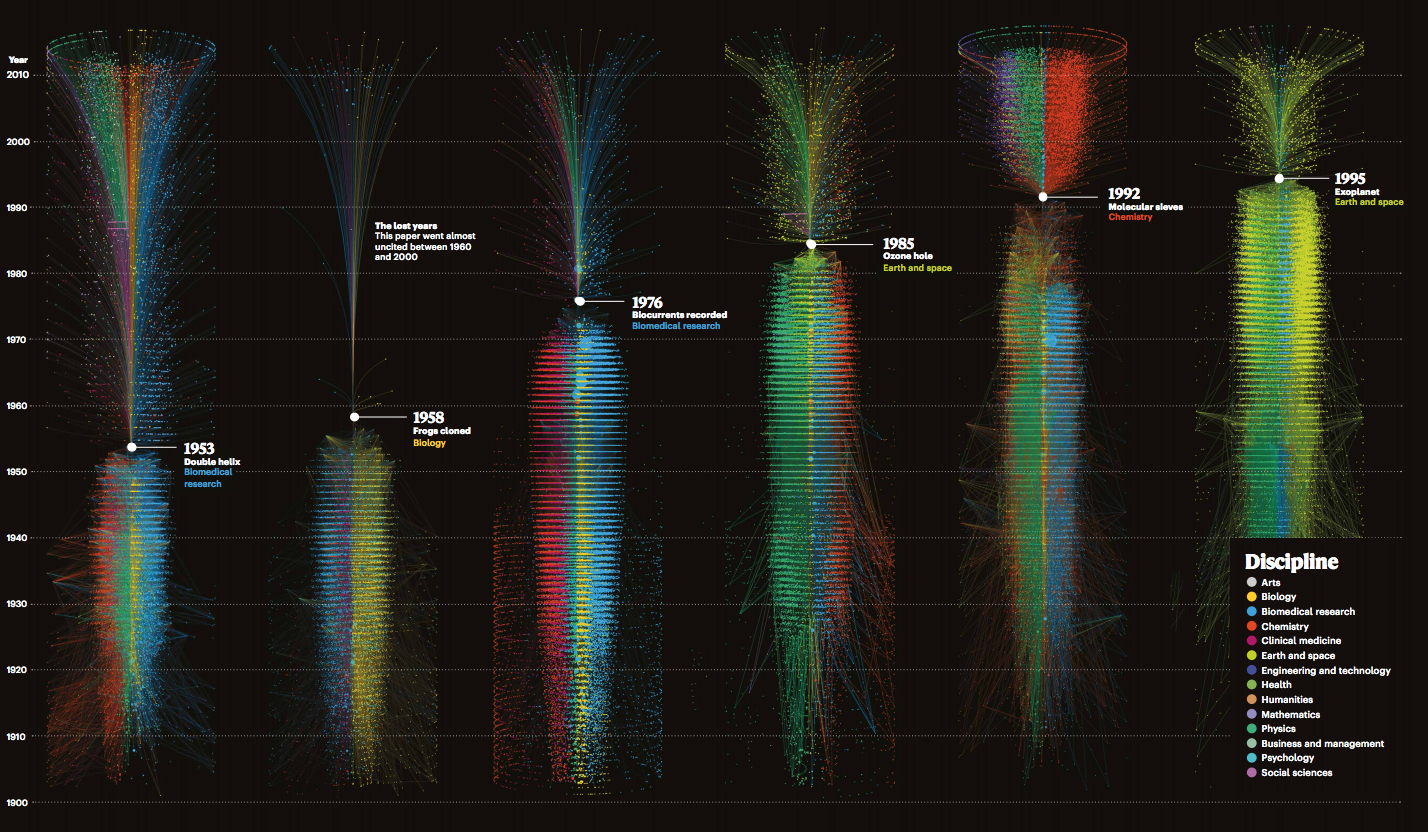
\includegraphics[width=0.92\textheight,angle=90]{figures_c3/naturegraph.png}

        \caption{\textbf{150 years of letters to Nature.} A visualisation showing how previous research is used to inspire future studies. Important discoveries (DNA, Cloning(frogs), Bio-Currents, Ozone Hole, Molecular Sieves and Exoplanets) are split into research which contributed to their formation (below), and the consequent papers produced from each discovery. Use of colour is used to emphasise the multi-disciplinary nature of prolific scientific discovery. Source: \citep{naturecover}}
        \label{fig:naturecover}
\end{figure}



\subsection{Data Collection}\label{sec:scholar}

To generate a dataset on papers related to the MCM. The academic search engine (Google Scholar \citep{scholar}) is queried for all articles containing the words \{ \emph{"Master", "Chemical", "Mechanism"} and \emph{"MCM"} \}. For each match, the first 100 pages of results are selected. Each of these contains 10 articles, from which the first 100 pages of related articles are chosen.
In taking the top 1000 citations for each page a network of 15744 papers and 30178 citations\footnote{Note: this had the potential of returning up to 1000,000 nodes} is created. This process made use of an edited version of the  \emph{etudier} Github repository, \citep{web}.


\subsection{Visualising the data.}

The initial visualisation of the dataset is accomplished through the use of THREE.js \citep{threejs}. This makes use of WebGL bindings and allows for the efficient viewing, querying and interacting of the data in 3 dimensions. This helped identify the temporal changes within the network by mapping a papers publication year to the $z$ direction, \autoref{fig:weball}, as discussed in \autoref{sec:filter3d}. 

\begin{figure}[H] %dont leave blank lines between sfig
     \centering
     \hfill
     \begin{subfigure}{0.495\textwidth}
         \centering
         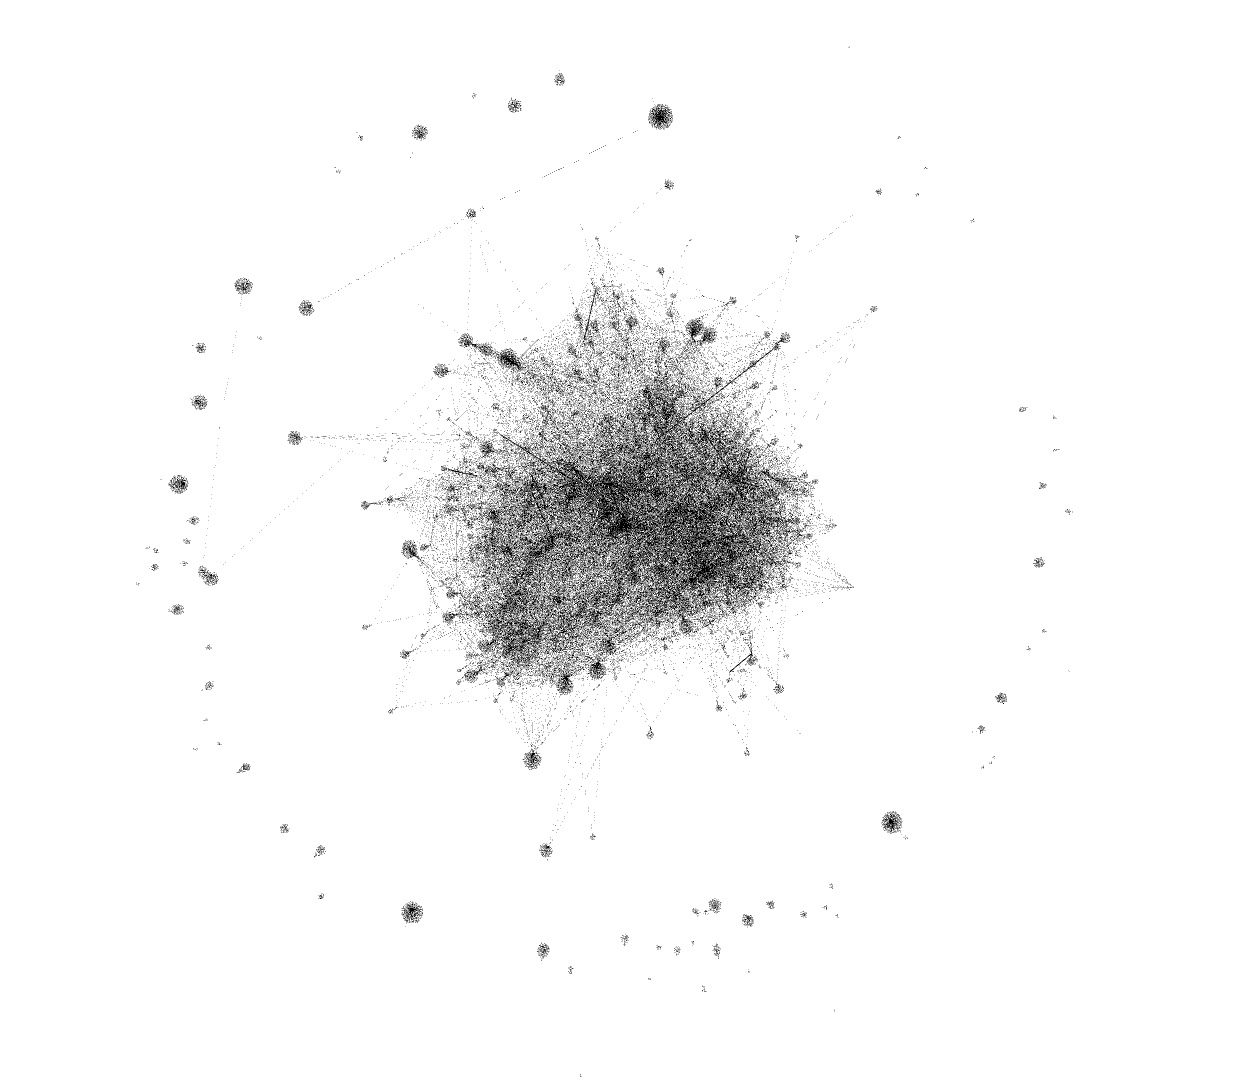
\includegraphics[width=\textwidth]{figures_c3/gephiall.png}
         \caption{A 2D force directed representation of the network using the gephi software \citep{gephi}}
         \label{fig:gall}
     \end{subfigure}
     \hfill
     \begin{subfigure}{0.47\textwidth}
         \centering
         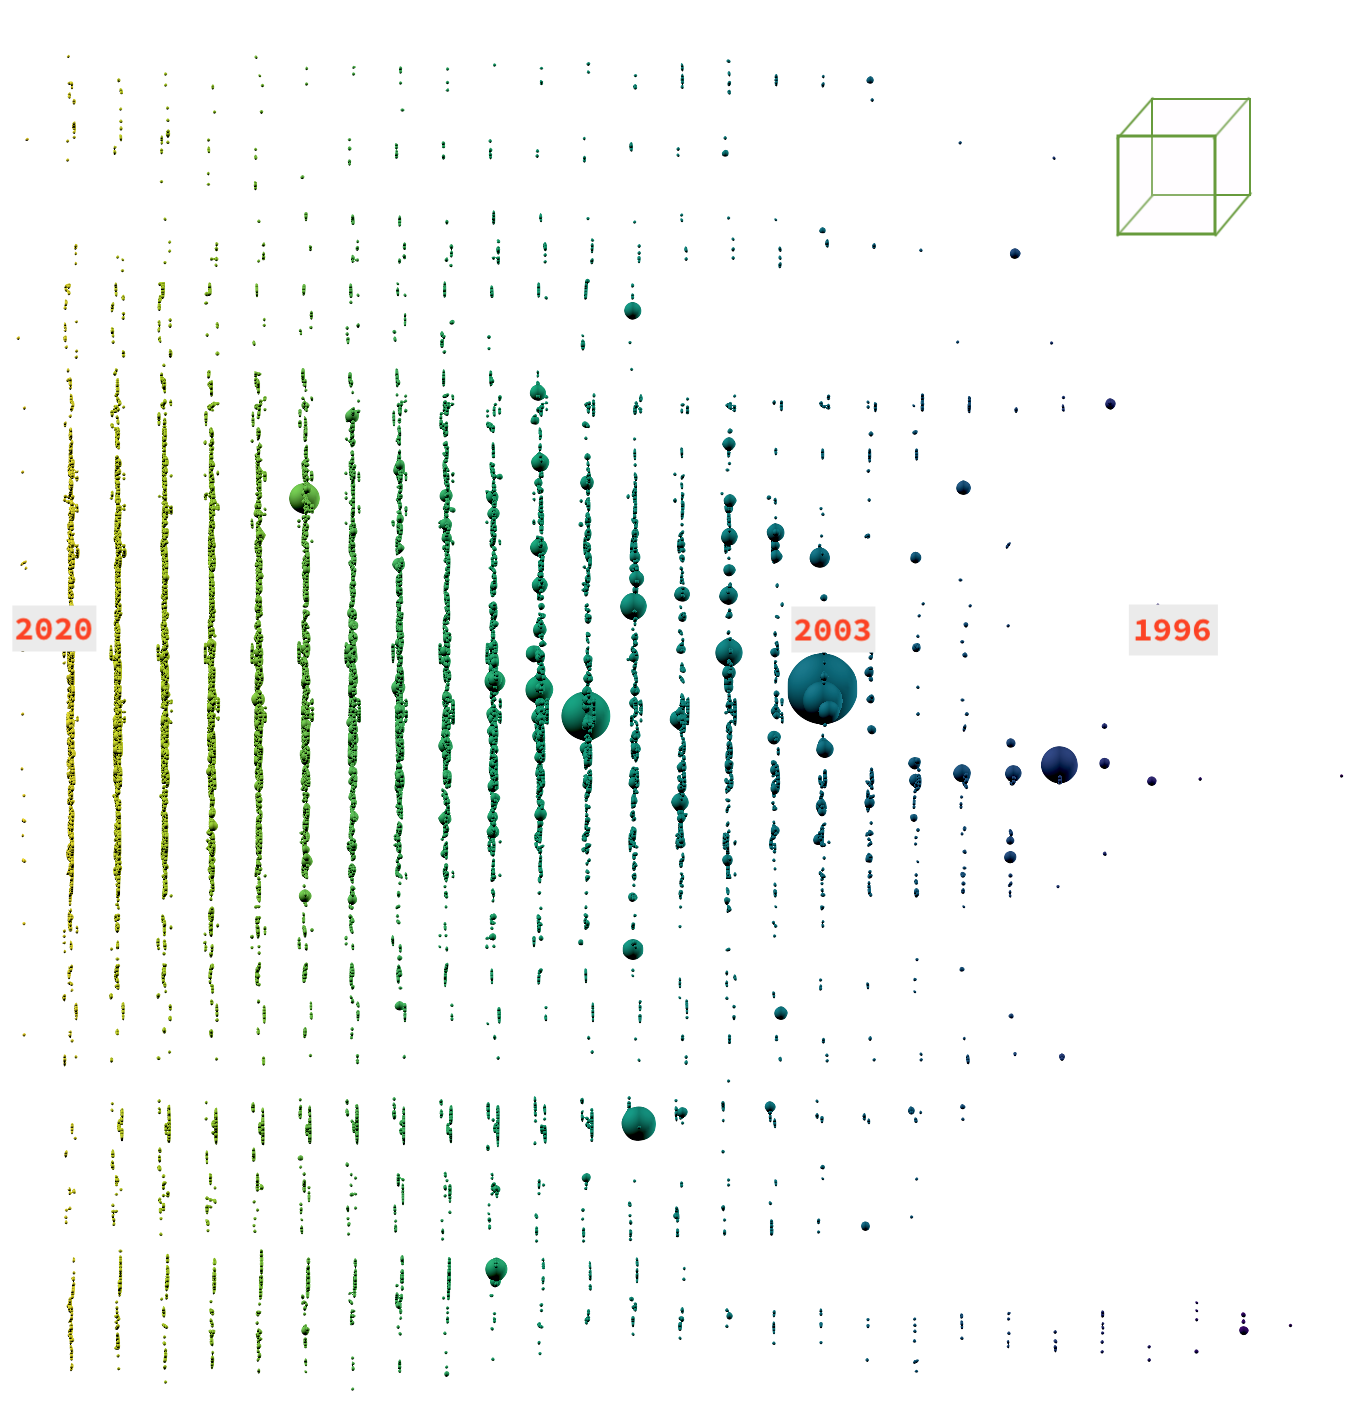
\includegraphics[width=\textwidth]{figures_c3/sideall.png}
         \caption{3D orthographic camera (sideview)}
         \label{fig:sideweb}
     \end{subfigure}
     \hfill

     \begin{subfigure}[b]{0.75\textwidth}
         \centering
         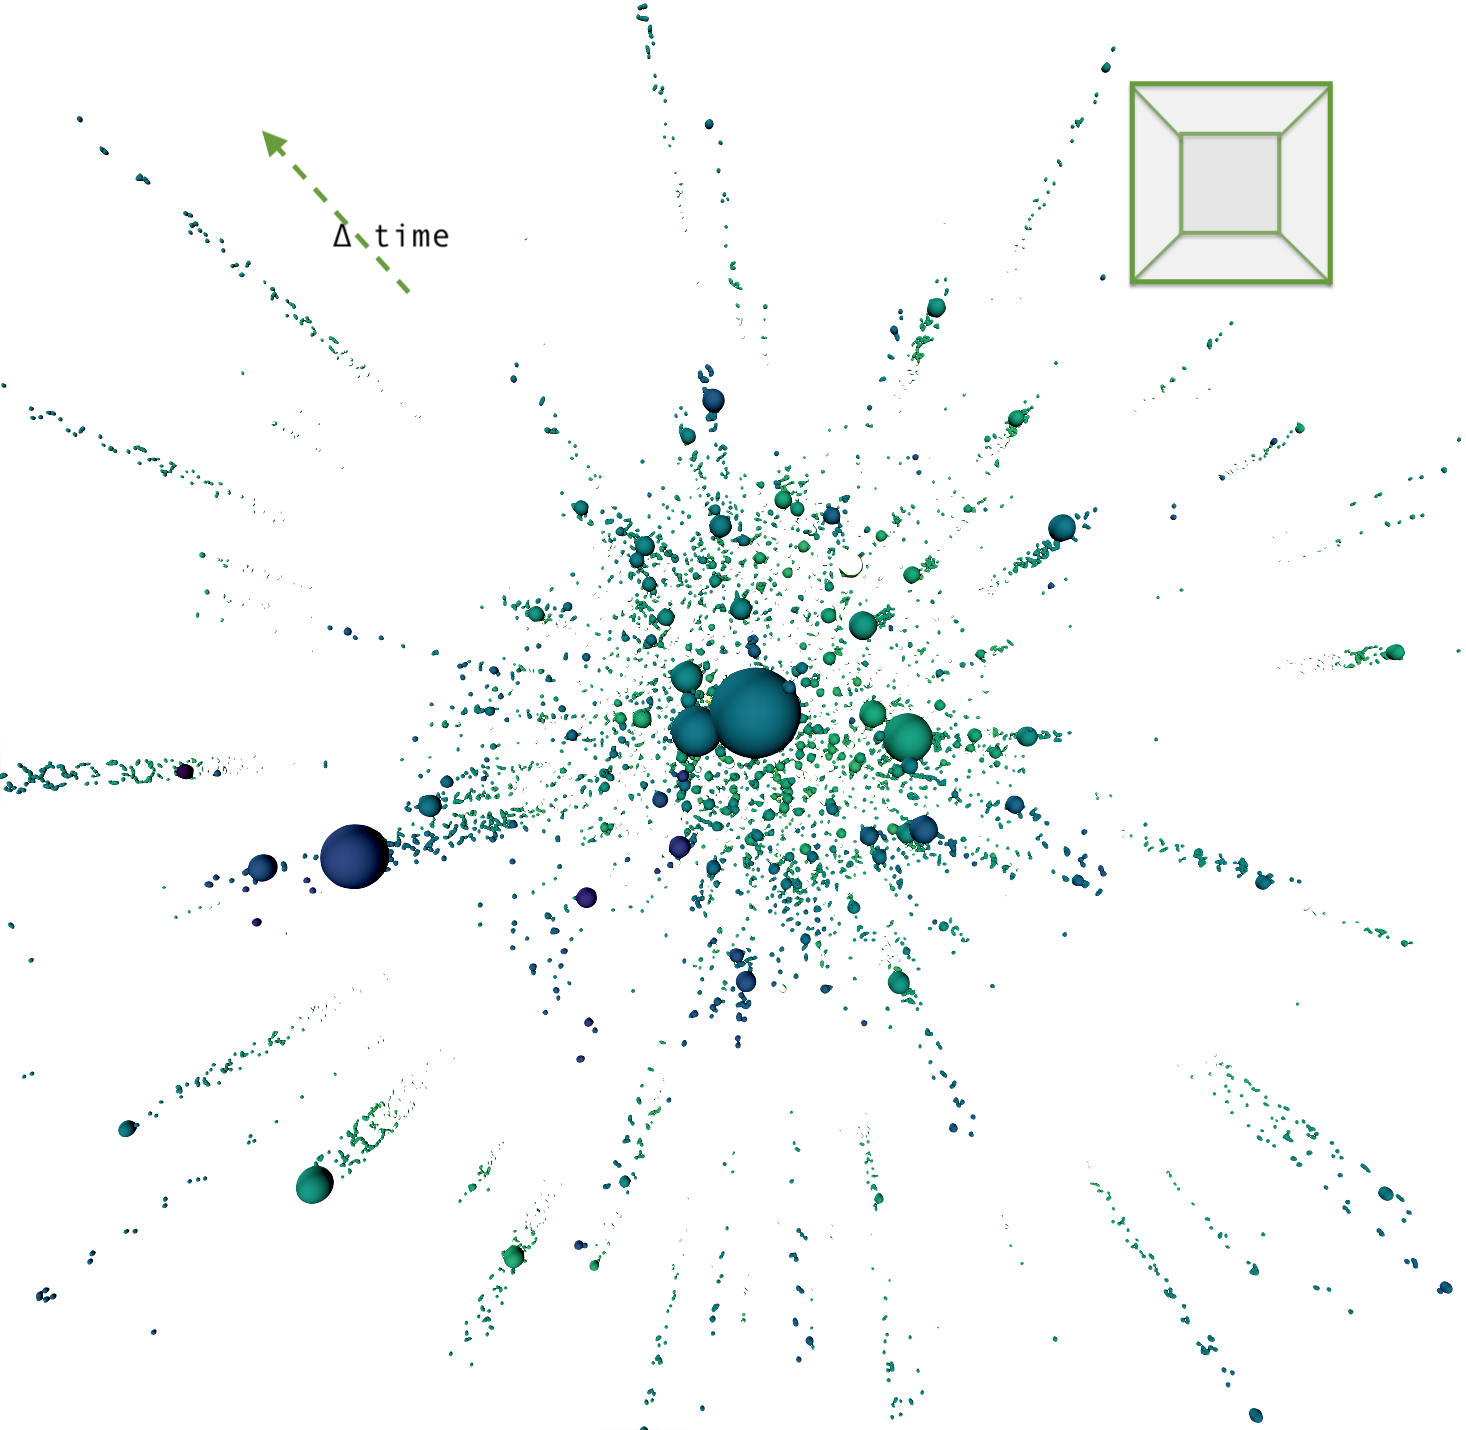
\includegraphics[width=\textwidth]{figures_c3/threeall.png}
         \caption{3D perspective camera}
         \label{fig:3dgeph}
     \end{subfigure}


        \caption{ \textbf{Initial 3D graph representation of the scraped MCM citation graph.} (a) shows the `classic' graph representation of the network. (b) shows a size representation using an orthographic perspective. Here time is shown across the $x$ axis, with yellow being the most recent. (c)
        uses a perspective camera, which emphasizes the...
        Still captures of 2D and 3D visualisations of the dataset. Node size corresponds to the number of citations, and colour (and z-axis) corresponds to the publication year for each paper.}
        \label{fig:weball}

\end{figure}


\subsection{Filtering the data}\label{sec:filter3d}


In the method used to web scrape data, there are several features which need to be corrected/removed. The reasons for this are discussed below.
 
\paragraph*{Pre-1996}
There exist several papers predating the conception of the MCM (1996). A number of these can be attributed as incorrect data, with publication dates <1900 which may be the result of missing information or a fault in googles web scraping algorithm. Any such papers are removed from the dataset.

 For otherwise correct articles, those published pre-1996 are also filtered from the dataset - this is because we are interested in identifying the influence the MCM has had on research and not the research that may have led to its creation. This can be seen in the cone-like shape emanating from the first MCM papers in \autoref{fig:sideweb}.

\paragraph*{N-th degree research}
Not all research articles in a field reference other articles with the same field. \autoref{fig:naturecover} showed us that many of the great discoveries in science have a multidisciplinary nature. It is for this reason that it is expected that articles from non-atmospheric areas of research may reference or build upon specific areas of research touched by the MCM. Such papers, and in consequence the papers which cite them, have little or no links to many of the core MCM papers. Such papers manifest themselves as a halo of satellite clusters which are connected by themselves but not with the main body of the graph, \autoref{fig:gall}. In using a 3D perspective viewpoint (\autoref{fig:3dgeph}) it is possible to identify the paper which references the MCM and then the consequent papers which cite it by observing the satellite clusters, and the gradually lightening spiral of papers which emanate out of it. 

Analysis of the network connections for each cluster can allow us to identify the indirect relationships some of these diverse topics (\autoref{table:otherpapers}) contained within the satellite nodes. Here it can be seen that the use of photochemical ozone creation potentials \citep{milk1,milk2} are used for the Life cycle assessment of Italian high-quality milk production \citep{milk}. 
Similarly indirect paths such as the paper:
 "Temporal controls on dissolved organic matter and lignin biogeochemistry in a pristine tropical river" (\citep{biogeo}) can be used to link to \citep{georiver1} and ultimately the MCM protocol paper \citep{mcmpartA}.
 
 If we desired to remove such papers, the simplest method would be to recreate the graph into one where links are drawn between papers that are cited together (\autoref{sec:cocitep})
 and then removing any nodes without any external connections (isolates).

\begin{table}[H]
\begin{center}
\begin{tabular}{ p{0.6\textwidth}|l }
 \hline
   & \\
 Fabrication of Bioinspired Actuated Nanostructures with Arbitrary Geometry and Stiffness & \citep{nano} \\ \\
 %
 Temporal controls on dissolved organic matter and lignin biogeochemistry in a pristine tropical river  & \citep{biogeo} \\ \\
Neuroproteomics in Neurotrauma & \citep{neurotrauma}\\ \\
%
Fast start-up of a pilot-scale deammonification sequencing batch reactor from an activated sludge inoculum & \citep{pilot} \\ \\
Red blood cell oxidative stress impairs oxygen  delivery and induces red blood cell aging & \citep{blood} \\ \\
%
Life cycle assessment of Italian high quality milk production. & \citep{milk}\\ \\
%
 \hline
\end{tabular}
\end{center}

\caption{A selection of research papers not directly connected to the field of atmospheric modelling.}
\label{table:otherpapers}
\end{table}



\paragraph*{Unprobable occurances}
Finally, the extracted network also contains many disconnected component subgraphs - graphs with no connection to atmospheric science. An example of this is seen in an article about neuroproteomics in neurotrauma \citep{neurotrauma}. In analysing the paths which connect this, it is seen to cite the paper on "Large scale gene expression profiling of metabolic shift of mammalian cells in culture", \citep{neuro2}. This is an anomaly which within its structure contains the words "Master", "Chemical" and "Mechanism" (separately) and has `MCM' as an abbreviation for one of the author names. To remove such papers, all disconnected sub-components are removed from the analysis. 



\paragraph*{A note on unintentional filtering}

\textit{
Author names and some extended titles may be truncated with the use of ellipses. This is due to the web scraping script extracting these directly from the Google scholar page, and not the original articles themselves. It is worth noting that the results in this section are not explicit, but rather a demonstration of graph theory on a real-world dataset.
}


\subsection{The Co-citation Network}\label{sec:cocitep}

The document coupling techniques of co-citation was introduced in the 1970s as an alternative approach for quantifying the results within the science citation index \citep{cocite}. Rather than representing a graph using backpropagation (through the use of referencing and citation counts), a co-citation network introduces a link between papers if, and only if, they have been cited together. Although this loses the directionality of a graph, it allows us to show forward propagating trends between papers within the same field. 

Applying the above method allows us to reduce the citation graph of 451 papers and 5402 edges to an undirected co-citation graph of 2758 edges - halving the number of original links between papers. 

\subsection{The Co-authorship network}
An alternative to exploring which papers which are cited together are to look at their authors. Here undirected links are drawn between authors on the same paper. This style of analysis was used to show that the number of papers per author, and the total number of authors per paper can vary between research fields, \citep{newmancoauthor}. In combining this with a series of network centrality metrics, \citep{coauthornew} revealed that it is possible to discern promising researchers from both iter and Intra disciplinary groups. 

In building a co-authorship network for the MCM, we can identify authors who publish together\footnote{ Disclaimer: as mentioned earlier, not all authors for every paper were recorded by the web scraping algorithm} and highlight research groups who work with the MCM, \autoref{fig:authorgroup}. This shows how authors with a similar geographic location/institution are more likely to publish together. The largest cluster here falls under the MCM developer team, which resides between the Leeds and York universities. Next two German institutions which are heavily involved in the atmospheric chemistry field (Julrich and Max Planck), followed by an assortment of Chinese authors, mainly centred around the Beijing or Hong Kong region. 


\begin{figure}[H]
     \centering
         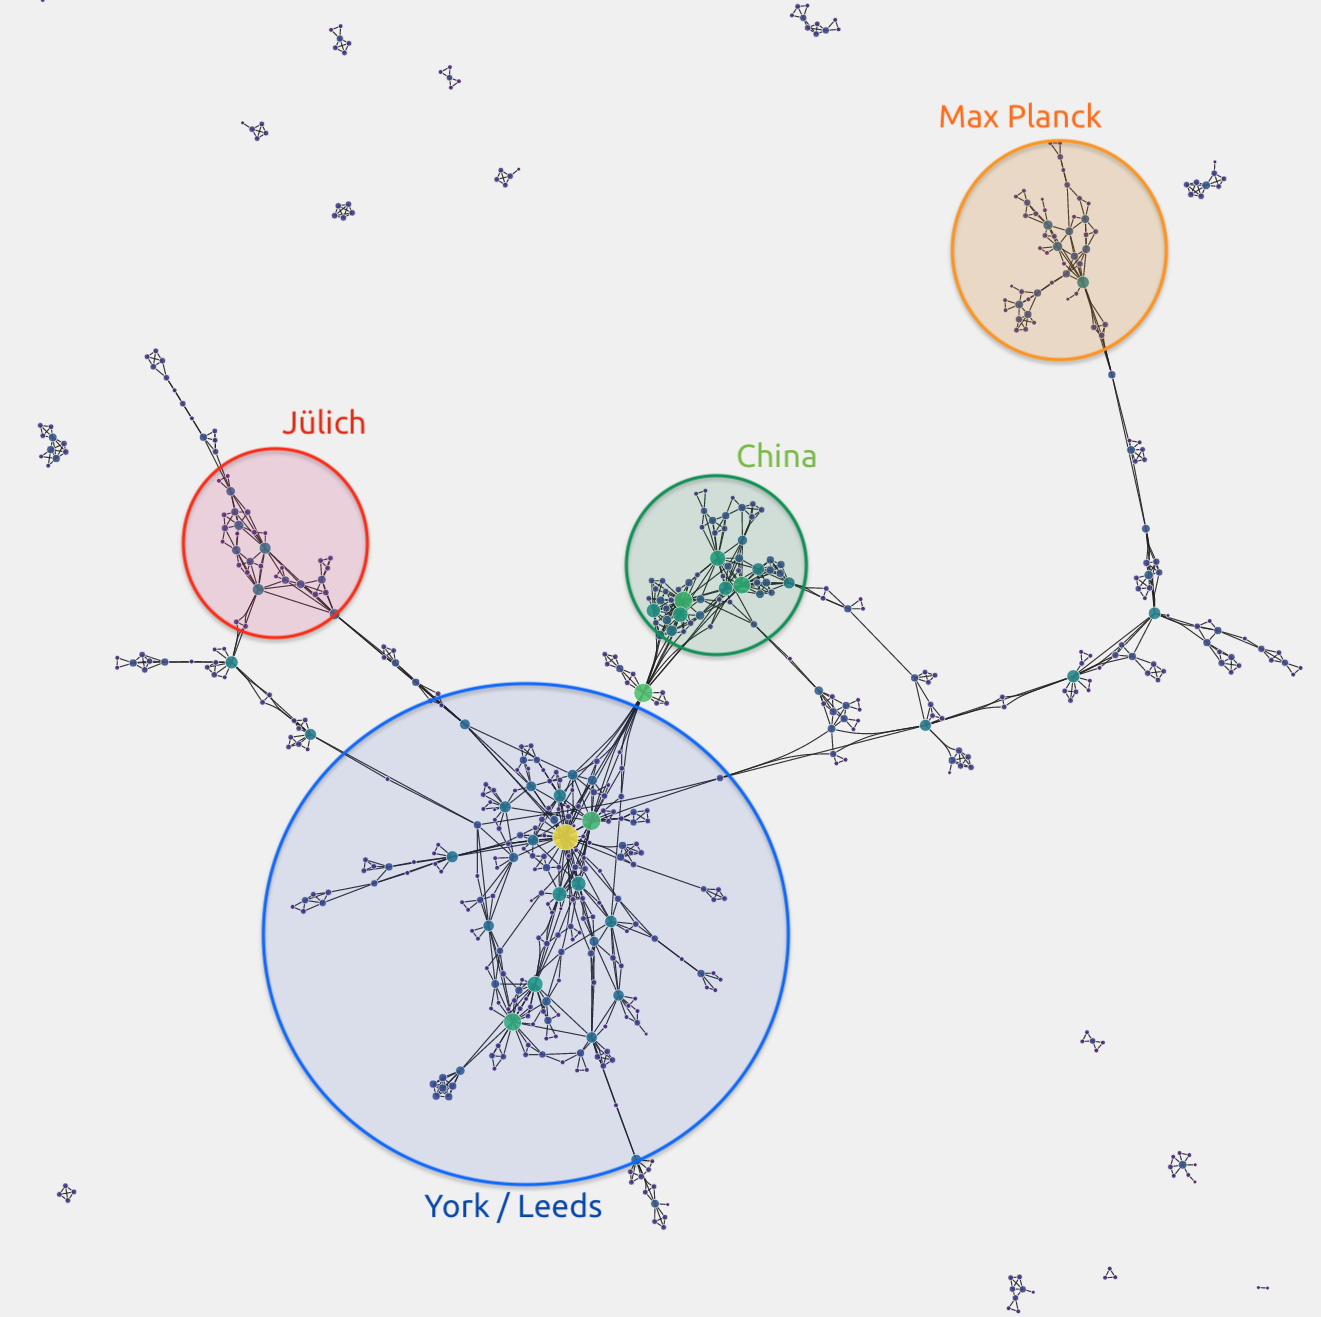
\includegraphics[width=.8\textwidth]{figures_c3/GroupAuthor.png}
        \caption{ \textbf{The co-author network.} In representing the authorship network as a force directed graph we are able to see cliques or clusters of people who publish together. It can be noted that this often occurs when they have a similar geographical location.}
        \label{fig:authorgroup}
\end{figure}



%%
%%%
%%
%
\section{Presentation and plotting.}
The simplification and visualisation of the MCM subset of N species and X reactions representing the chemistry within Beijing during the summer of YYYY is presented. We use properties of molecule structure and functional groups to partition species into like groupings. This is done through mechanistic network representation (force graphs), linear mathematics (principal component methods), force-like visualisation (t-SNE and UMAP) and neural network auto-encoders. For each example, several types of possible inputs are used, and the output reduces to two dimensions for visualisation. Each DR model can be fine-tuned to produce optimal results, however, due to the time and length constrictions of this chapter arbitrary values similar to those used by default have been chosen for the input parameters. It is taken that this section aims to juxtapose the many methods as a means of determining which may be suitable for the clustering of measured/simulated data (Chapter NEXT).

\subsection{Visualisation}
Once reduced to two dimensions the results are plotted using two different methods (outlined below).

\subsubsection{Graph visualisation}
To represent graphs we take an approach similar to previous chapters. Here nodes are represented as circles, sized according to the number of functional groups or the amount a specific group exists. To reduce clutter links between spatially distant species are bundled (\cite{edgebundle}), whilst those close together are not changed (a technique similar to that used in \cite{graphtsne}. Nodes are assigned properties and may be matched using full or partial matches to their names, functional groups or smiles strings. Interactivity through the use of mouseover events are used to accomplish the level of exploratory data analysis required for this task.

\subsubsection{Latent Space / Embedding visualisation}
When data is reduced to two dimensions, we may represent it in the form of an x-y scatter plot. To do this, we first normalise the model output such that it lies between 1 and 0. This removed the need for axis and allows us to compare different outputs directly. As an indicator node groupings are clustered using the DSBSCAN algorithm from sci-kit learn \cite{scikit,DBSCAN}. This selects nodes residing between the maximum distance of 0.02 between the two samples (dimensions. Here trends are once again hi-lighted and labelled with the use of automated and manual exploration aided by interactivity.

\paragraph{Four Colours Theorem}
When plotted, the number of clusters detected often exceeds the number of categorical colours available. In an attempt to reduce these we apply a greedy implementation of the four colours theorem \cite{fourcolour}.
The four colour theorem states that each map may be coloured with no more than 4 colours. More explicitly than any two regions (e.g. a country if we are looking at world map may not share the same colour as this causes ambiguity between results. This is especially true when trying to visually differentiate different clusters by colour. The algorithm developed uses the Delaunay tesselation scripts contained within DataDrivenDocuments.js (d3js) \cite{d3js}. This partitions our plane into polygon-regions with boundaries at the furthest distance from each point (Voronoi cells) \cite{delaunay}. Using this we may start at a randomly assigned cell providing it with a colour. We then recursively iterate through all neighbours assigning them with the lowest possible colour that does not occur within any of their neighbours. Although such a greedy approach does not produce an optimum result it allows for the colouring of data with $\le 5$ distinct colours.


\qfig{4fig/4colour.png}{fig:4col}{An example 4 colour matching using the first implementation of the above algorithm - Observable Notebook : \cite{4colobs}}{.7\textwidth}

\paragraph{Exposing data}
Since much of the initial exploration was done using manual intervention and interaction, we found clusters of nodes would often occupy the same space within a graph. There exist two solutions, one of which involves reducing the size of the dots to prevent overlaps, however, this does not always prove useful and often results in difficulties when trying to select a node. The alternative is to apply the d3 force-directed algorithm combined with a level of collision detection. \\

Nodes are configured in such a way that experience a strong attraction force to their respective $(x,y)$ coordinates. The collision algorithm then repels them from existing within the radius of other nodes. This transforms any clusters of stacked nodes into adjacent groupings around the common centre, in turn making it possible to select each node individually.

\paragraph{Gooey Effect (Gaussian Blur)}
When comparing the existence of certain properties it is often to use colour as an encoding. To prevent distraction through the recognition of separate points, it may be found that blurring adjacent points into a single mass whilst representing information of interest using a variable colour gradient, reduces the cognitive load on the end-user (especially when it comes to dense plots consisting of multiple points.

The simplest way to do this is to apply a gooey-style filter (a method used for creating water droplet style effects in web animations). This works through the merging of ... and a Gaussian blurring matrix of INSERT HERE.


\section{Results}

\subsection{The Network Approach}

The oxford dictionary describes a network as `a group or system of interconnected people or things' \cite{definenetwork}. Such an idea may be applied to a chemical system through representing species as our nodes or items and the reactions that exist between them as the interconnected links binding them together. This analogy lends itself to not only producing a holistic representation of how species are related to each other but the use of visualisation in determining like properties.

\subsubsection{Visualising the Mechanism}

A chemical mechanism contains all\footnote{Sometimes this may be all probable reactions concerning a research aim.} possible reactions between a subset of species. It, therefore, follows that information about the structure of each species has been used to determine the existence and rate of a reaction. Since reactions may be broken down into reactants and products, it is possible to construct a node-link style directional graph with links going from each reactant to each product.\\

In using a type of force-directed algorithms, we apply the OpenOrd layout \cite{ord} to the subset of chemistry derived from the YYYY Beijing campaign [REF!]. This uses a combination of simulated annealing\footnote{A method inspired by metallurgy where the material is slowly heated and cooled to remove internal stresses} and edge cutting to overcome local minima and produce visually distinct clusters of highly connected nodes, \autoref{fig:graph}.

\qfig{4fig/graph/n_carbons.png}{fig:graph}{A graph representing the Beijing data set described in XX. Colours represent the number of carbons for each species (light == more), and node size shows the number of functional groups. }{.9\textwidth}





\subsubsection{Functional group location within the graph}

Carbon - Hydrogen chains are the backbone of all organic chemistry. Alkanes are saturated hydrocarbons which are unlikely to react. If we remove hydrogen, we free up an electron and form an unsaturated alkyl chain. With the addition of a functional group, we increase the reactivity of such a species, making it more likely to form a bond with something else. This is called functionalisation. Comparing \autoref{fig:graph} and \autoref{fig:graphother} we see that in general, as the number of carbons decreases, the number of non-carbon atoms increases. This may be explained through the iterative oxidation of primary emitted carbon chains, to ultimately produce \ce{CO2} and water (not shown on the graph)\footnote{Carbon monoxide is located at the centre of the graph where all the links converge. Although the MCM does not explicitly include carbon dioxide, one of a hand full of channels from which this forms involves a reaction with \ce{CO}, which is why so many reactions go into it}.

\paragraph{Reactivity and the Graph}
Within the field of geochemistry van Krevelen diagrams are commonly used to to show the evolution (and in turn oxidation) of coal and oils.

This is done through looking at the ratio of Oxygen to Carbon and Hydrogen to Carbon within a specific species - the notion being that in oxidation, Hydrogen-Carbon links are replaced with Oxygen [ADD LIST OF REFS HERE - original paper hard to find]. In looking at such ratios, we may evaluate the extent of oxidation a species has experienced and draw parallels between their relative structural significance.  \cite{krsig}.

To confirm our hypothesis that the chemistry within the graph begins with large hydrocarbons, which are then oxidised in a cascade of reactions to ultimately form \ce{co} we may colour nodes using the total possible O-C ratio. This can be calculated as by:

\begin{equation}
    Ratio = \frac{O-C \ bonds}{Total \ potentially  \  available \ H-C \ bonds.}
\end{equation}

Since it is structurally improbable that all hydrogen's in a carbon chain are replaced by Oxygen, there are fewer values within the (top) yellow range of the colourmap, \autoref{fig:ocratio}. However is is evident that in general the closer we get to \ce{CO}, the higher our O-C:O-H ratio.

%
%\qfig{4fig/graph/n_other.png}{fig:graphother}{A graph representing the Beijing. Hilighted colours represent the number of atoms other than carbon within a species (light == more). Node size shows the number of functional groups. }{.9\textwidth}
%
\qfig{4fig/graph/oxidised_ratio.png}{fig:ocratio}{Oxidised ratio - the percentage of all possible oxidation }{.9\textwidth}





% We may further explore the groups presented in \autoref{fig:graph} by viewing the location of species containing different functional groups. Since


\paragraph{Graph Embeddings and Multifunctionality}
\autoref{cover} shows that species in the MCM often have multiple possible functional groups, each of which may react with different species. We know that species in a mechanism are connected with regards to their reaction. We are interested to see if these are separated within the force directed graph layout. Upon initial inspection (through the use of manual interaction) similarity between both naming convention and smiles strings exists within the graph, \autoref{fig:graphnames} and \autoref{fig:graphsmiles}. Here an example subset of some of the matches found using the javascript document query matching function are shown.

%$^$ denotes the start of the string, .$*$ a match anywhere and $\$$ at the end.


\qfig{4fig/graph/namegraph.png}{fig:graphnames}{Partial name matches for species within the network}{.9\textwidth}

\qfig{4fig/graph/smilesgraph.png}{fig:graphsmiles}{Partial smiles matches for species within the network}{.9\textwidth}


From this we start to build a picture - we know that that as species react, much of the time we alter a bond or functionalisation, whist retaining the general structure of the molecule. Many reactions are also cyclic, with for example an alcohol being lost, and then reattached again. Additionally like structures will have similar reaction patterns, and very likely react with the same species / inorganics. Since force-directed graphs rely on links between items to produce the final embedding, it serves that such features constrain connected species towards a common location - for example the Aromatic region (orange *c in \autoref{fig:graphsmiles}).\\

Since reactions are gouverned by functional groups, we wish to see if such information may be extracted from the structure of the mechanism. Functional group abundance for each species may be calculated to provide the percentage of species in the graph that should contain it \autoref{tab:percentfunctional}. In the next section we look at each functional group, how it reacts and their distribution across the subset and graph.

\begin{table}
\begin{tabular}{lr}
\toprule
Species Name &  Percentage likelyness \\ \midrule

Alcohol        &   52.91\% \\
Ketone         &   42.61\% \\
Aldehyde       &   20.10\% \\
Nitrate        &   13.60\% \\
Peroxalkyl rad &   11.49\% \\
Alkoxy rad     &    8.40\% \\
Aromatic rings &    5.40\% \\
Ether          &    4.34\% \\
Ester          &    3.93\% \\
PAN            &    3.24\% \\
Carb. Acid     &    1.92\% \\
Per. Acid      &    1.65\% \\
Criegee        &    1.61\% \\
\bottomrule \\
\end{tabular}

    \label{tab:percentfunctional}
    \caption{Percentage probability of a species at random from the extracted subset containing each functional group. }
\end{table}




\paragraph{Alcohol: R-OH}



An alcohol can be described as a species containing the hydroxyl functional group (\ch{OH}). These are very common in organic chemistry due to their simple formation (the addition of Oxygen to an unpaired electron). \autoref{fig:graph_Alcohol} shows species containing the functional group are evenly distributed throughout the mechanism. The two most common reactions for these are

\begin{equation*}
R:OH \rightarrow{{+OH}} R:O.
\end{equation*}

\begin{equation*}
R:OH \leftarrow{~hv} R:O.
\end{equation*}

and

\begin{equation*}
R:OH \rightarrow{{+NO_2}} R:=O (+NO)  \rightarrow{{+ ~hv|NO_3|OH}} RO.  \rightarrow{{+HO_2}} R:OH (+O_3)
\end{equation*}

Reactions of species containing an alcohol group often do react with other available functionalgroups.


\paragraph{Ketone: R-C(=O)-R'}
Ketones consist of an aldehyde chain containing a carbonyl group. Ketones are thought of simple functional groups as the carbonyl is not paired to another functional group (e.g. Carboxylic Acid or Esters). These are again common throughtout the mechanism and do not local to a specific group of species, \autoref{fig:graph_Ketone}. \\

The most common reactions are...

Everything or not at all?


\paragraph{Aldehyde: R-C(=O)H}
Aldehydes consist of a formyl functional group (a carbon double bound to an oxigen and singly bound to a Hydrogen), and may often be found in essential oils. This functional group makes them more reactive...
When observing \autoref{fig:graph_Aldehyde} we see that many of the aldehydes appear within the central cluster, (around Carbon monoxide where many of the shorter length and more oxidised species are). There is another grouping just above this, where the benzine derivative exist. On the left many of the aldehyde grouping are part of large (6/7) long carbon chains containing only Hydrogen and oxygen. It is worth noting that within the graph, Formaldehyde (\ce{HCHO}) is located at the nexus, left of centre. Similar to this many of the aldehyde groups appear to exist within species containing many reactions between themselves, and to others. \\





Aldehydes are often generated t



\paragraph{Nitrate: R-O-\ce{NO2}}




These are relatively well distributed throughout the graph and commonly react with both Aldehydes and Ketones, which are both also well distributed and in abundance, to convert these into alcohol or PAN groups and Nitrogen dioxide. The most likely reaction pathways for this would be \\

 THe cluster INB1NBCO3H and INAHPPAN derviatives?
This is clear withinin .. .


\paragraph{Peroxalkyl Radical: R-O-OH}
Common





\paragraph{Alkoxy Radical: R-OH }

This is an alkyl chain (Carbon and Hydrogen) bound to a single Oxygen group.


\paragraph{Ether: R-O-R'}

Ethers are two alkyl (Carbon and Hydrogen) groups joined by a single oxygen. These have relatively low boiling points and have an aplication in the removal of alcohol functional groups through binding with the oxygen and expelling the hydrogen. Their ---- nature places them in close proximity to aromatic and PAN clusters on the graph.


\paragraph{Ester: R-C(=O)-O-R'}
Esters are compounds often derived from acids, in which at-least one OH group is replaced by an -O-alkyl (Carbon and Hydrogen) group. This suggests a similar reactivity style to ethers....

\paragraph{PAN: R(=O)-O-O-N(=O)O}

A secondary pollutant which is thermally unstable and decomposes to form \ce{NO2}. Peroxy Acetyl Nitrates are a found within photochemical smog (ozone events) and are more stable than ozone. This makes them important when considering the long-range transport of smog related pollution.


\paragraph{Carb. Acid: s R–C(=O)-OH}
///
\paragraph{Per. Acid}
\paragraph{Criegee}






% \autoref{cover}


% \newpage
% Autoencoders :

% https://towardsdatascience.com/dimensionality-reduction-for-machine-learning-80a46c2ebb7e

% I\\


% http://mlexplained.com/2018/09/14/paper-dissected-visualizing-data-using-t-sne-explained/

%https://mlexplained.com/2018/09/14/paper-dissected-visualizing-data-using-t-sne-explained/

% https://gist.github.com/mbohun/3126926

%

\section{Introduction}

\subsection*{Historical significance}
The established process of trial and error has always underpinned our survival \citep{TrialandError}. Babies are born to rely on a set of sensory reflexes and a framework for physical reasoning \citep{pr}, and with these, we develop methods to navigate the influence of change within a physical, and auditory space \citep{objects}. This method of decision making is reflected in our adult lives with ideas and actions being limited in choice by our intuition and experience \citep{descartes}. In science, we apply a methodological framework consisting of a continuous assessment of scepticism, educated guessing (hypothesizing) and rigorous practical testing. Specialists accrue years of practical and theoretical knowledge within a narrow field and can identify areas of potential gain and futility. Yet even with all prior knowledge, the discovery of new and untested techniques involve the tortuous traipsing through a sea of uncertainty. Such a methods sometimes prove fruitful, through accidental discoveries of items such as x-rays, penicillin, etc. \citep{accidental}; finding novel applications for existing methods such as optical tweezers for chemistry or the abstract field of maths utilised by Einstein [REF], but more often than not end in the constant evolution of a pre-existing project with no clear result. 

\subsection*{Theory and Simulation in Science}

Until recently much of the experimentation possible was limited by resources, levels of knowledge available technology. With the increase of computation power, we have been able to not only increase our understanding but also run theoretical simulations to guide exploratory efforts with an impact on real-world applications \citep{dft,lion,theoreticalbio,drug}. However, as our ability to record and produce data increases, the need for the scientific method diminishes \citep{wired}. Here the application of `big data' tools and algorithms can provide insights and correlations much more compelling than the predictive capabilities of constantly changing models - ``Since all models are wrong the scientist cannot obtain
a "correct" one by excessive elaboration'' - \cite{allmodels}. As our level of attainable technology increases, so does the complexity of the data collected. Modern data-sets tend to be large, complex and highly multivariate. Although this greatly improves the quality of science that may be extracted from them, the difficulty lies in trying to represent it in such a way that we may successfully access the reliability of the results. Since simple bar and line graphs are no longer applicable, one solution falls within a class of unsupervised machine learning techniques called dimensionality reduction (DR).


\subsection*{Chapter Aims}
In \autoref{ch1} we looked at visual representation as a way of understanding complex systems. \autoref{ch2} showed that the chemical properties could be visually inferred from the node-link graph structure of a mechanism. Similarly, \autoref{ch3} and \autoref{ch4} located the presence of important species and clusters of like properties by applying mathematical algorithms to the graph network. As opposed to attempting to visualise complex data, this chapter looks at learning the structure of a chemical species and simplifying it into two dimensions. Here it is possible to extract key features of like-groups through the use of vector clustering, which unlike the graph clustering in \autoref{ch4} works by determining the density between points on a plane.  

The chapter begins with the introduction of the chemical system, and the various methods for representing species structure within it (\autoref{sec:drinput}). Next, we define the dimensionality reduction methods which shall be used to simplify the aforementioned inputs (\autoref{sec:dr}). This is followed by a brief overview of the visualisation methodology (\autoref{sec:visdr}). Finally, all three sections are combined to produce a set of result and conclusions about the use of DR to identify species structure.  

















%

\section{Species of the MCM and ways to represent them.}\label{sec:drinput}
The master chemical system (as defined in all previous chapters), represents our foremost knowledge of gas phase chemistry within the troposhere. It has been shown that due to its creation protocol (\autoref{fig:protocol}), much of the information about a species structure is encoded within the reaction pathways it can take. This section explores the different methods of representing a species structure, with the aim of providing a machine built algorithm with the greatest amount of information about each species and its functionality. To do this a range of input types will be evaluated against a number of different dimensionality reduction algorithms with the aim of isolating which chemical properties are most `picked up'. 

\subsection{Input generation}
The MCM provides species information in the form of a species `smiles' (\autoref{sec:smiles}) and the IUPAC InChi string \citep{inchi}. Within this chapter we use only the smiles string, which is either manually processed using regular expressions or with the aid of pythons RDKIT package \citep{rdkit}. There are seven different methods for representing the chemsitry, each of which are outlined below. 


\subsection{Manual Categorisation}
Reactions within the MCM are determined by a set of rules (PROTOCOL SECTION). These are designed to mimic the process a chemist my discover new species, and often rely on the bond availability and functionalisation of a species. Since the present functional groups are the benchmark of whether a DR algorithm has sucessfuly separated species structure, it make sense to run a unit test using the known functional groups of a species as the input. 

To genearate the functional groups the regular expressions in \autoref{tab:fngroups} are used\footnote{To see the structure of each functional group type, go to \autoref{appendix:fngroups}.} on the smiles strings (described in \autoref{sec:smiles}) for each species. In extracting the functional groups we are able to plot the likelyness a species with a certain group is likely to have another using a chord diagram - \autoref{fig:covermcm}. Since most species are found to contain a multitude of functional groups, the separation of these into `tidy' clustered groups seems unlikely.      


%
% Except for dissociation, species reactions are often dictated by their functional groups. Species in the MCM are usually represented as functionalised alkanes (A saturated hydrocarbon in the form of $C_nH_{2n+2}$). In removing a hydrogen we form an alkyl chain. This allows for the potential of forming a bond with other atoms. By themselves alkyl chains are mostly un-reactive, however in gaining additional functional groups (functionalisation) their reactivity increases.%



\begin{table}[H]
    \centering
    \begin{tabular}{c|p{5in}}


PAN & \verb! C\\(=O\\)OON\\(=O\\)=O$|^\\[O-{0,1}\\]\\[N\\+{0,1}\\]\\(=O\\)OOC|!\\&\verb! O=N\\(=O\\)OOC\\(=O\\)|C\\(=O\\)OO\\[N\\+{0,1}\\]\\(=O\\)\\[O-{0,1}\\]!\\&\\

Carb. Acid & \verb! [^O](C\\(=O\\)O$|^OC\\(=O\\))!\\&\\

Ester & \verb! [\^O](C\(=O\)O\b|OC\(=O\))C!\\&\\

Ether & \verb! (\([\^O=]+\))*C(\([\^O=]+\))*O(\([\^O=]+\))*C(\([\^O=]+\))*!\\&\\

Per. Acid & \verb! c\\(=O\\)OO$|^OO\\(=O\\)C!\\&\\

% Hydroperoxide & \verb! COO$|C\\(OO|OO\\)C|^OOC!\\&\\

Nitrate & \verb! O(NO2\b|NOO\b|N\(=O\)=O|\[N\+\](?:\[O-\\]|\(=O\)){2})!\\&\\

Aldehyde & \verb! C=O$|^O=C!\\&\\

Ketone & \verb! C\(=O\)C!\\&\\

Alcohol & \verb-CO\\b|(?=^\\b)(?!^\\[)CO.|(?=^\\b)(?!^\\[)OC.|\\(O\\)|C\\)O(\\b|[^O]-\\&\\

Criegee & \verb! \[O-\]\[O\+\]!\\&\\

Alkoxy rad & \verb!\[[\/]{0,1}CH{0,1}\]|\b[\^O]\[O\.{0,1}\]!\\&\\

Peroxyacyl rad & \verb! \\ w\(=O\)O\[O\.{0,1}\]!\\&\\

    \end{tabular}

    \caption{CHECKKKKKKK!!!!!!!!!  A set of regular expressions that may be used to determine the number of occurrences of a functional group within a SMILES string.}
    \label{tab:fngroups}
\end{table}



\begin{figure}[H]
    \centering
    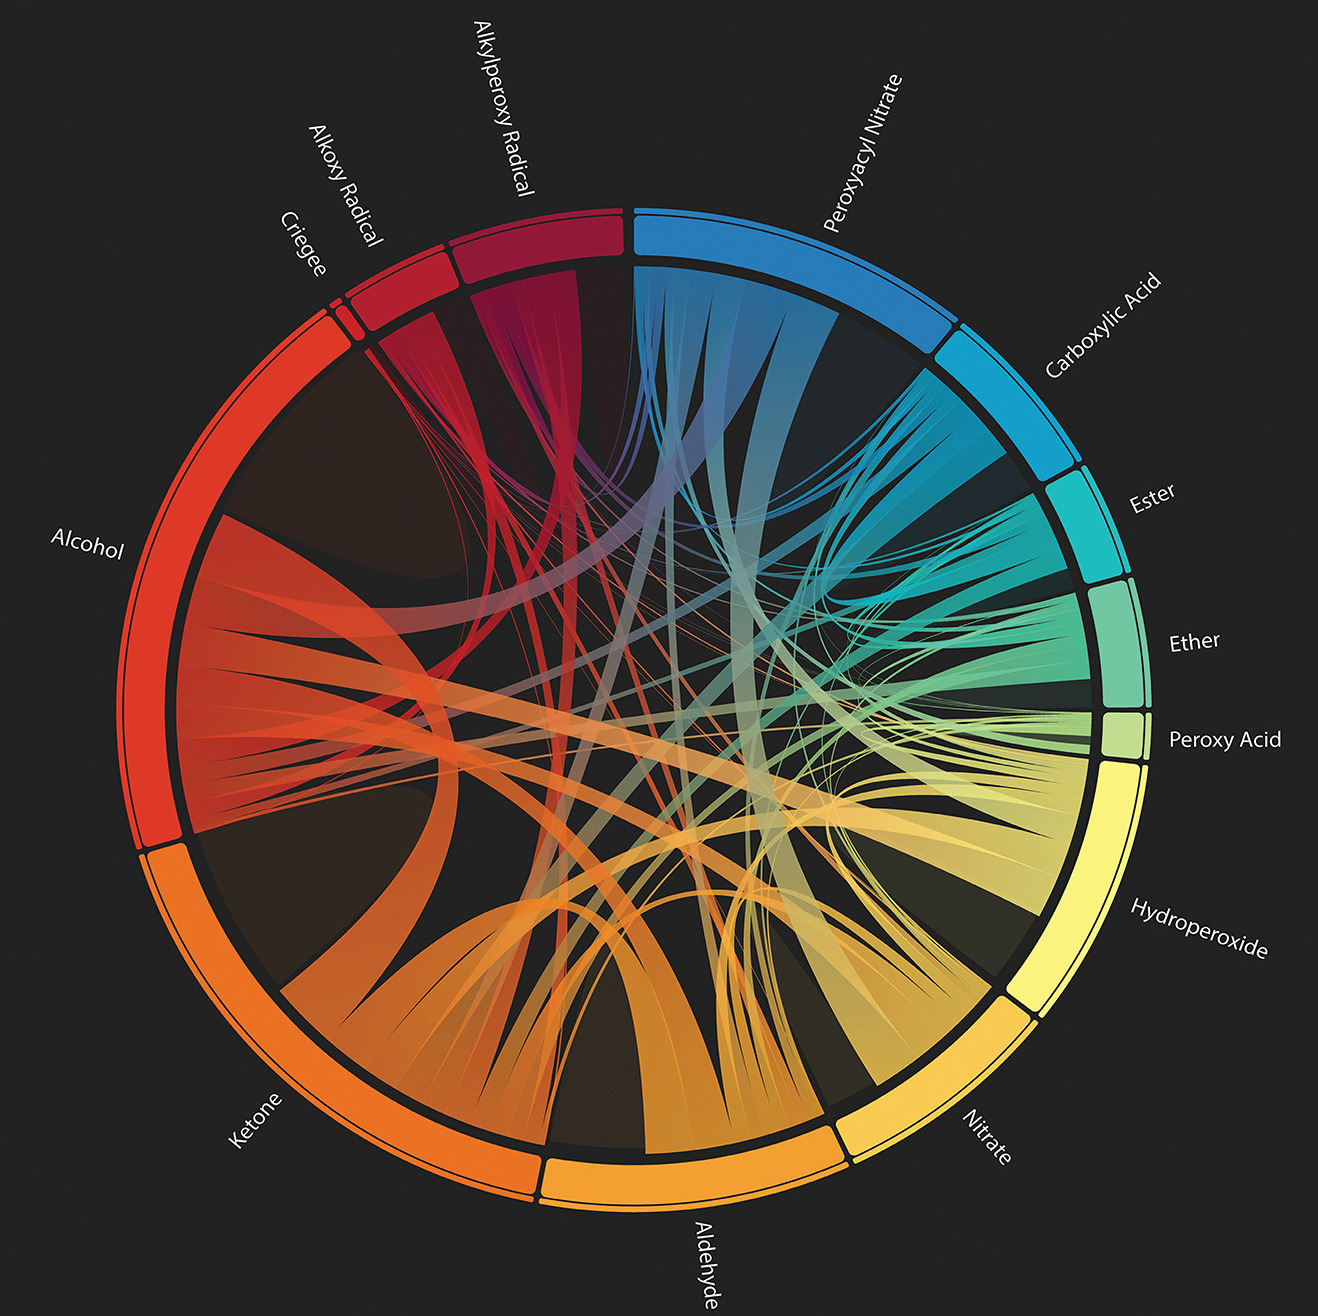
\includegraphics[width=\textwidth]{4fig/coverfig.jpg}
    \caption{\textbf{The multifunctionality of the MCM.} A chord diagram showing the functionalisatoin of a species within the MCM. Arc sizes represent what percentage of all functional groups in the MCM mechanism a group contains. Translucent areas of no outwards links represent species with multiples of a certain functional group, of which Alcohols and Ketones have the most.  
    Source: \citep{cover} }
    \label{fig:covermcm}
\end{figure}



\subsection{Tokenization}
As computer algorithms are unable to understand words, or their meaning, we have to first categorise the data into groups. Tokenisation is the conversion of a string into characters and representing them with a numerical equivalent. In doing so a string of characters can be converted into a numerical vector, allowing for its representation in a latent vector space. 
Within our input selection, we have two sets of inputs we can convert. These are the species names, and their smiles string representation. 



\subsubsection{Species Names}
In \autoref{ch4} it was shown that the dedicated species names for species in the CRI mechanism were often representative of their structural properties. This addage also applies for the MCM, where an intitive naminc convention has been selected. This is is often derrived as part of the construction protocol, where a species names reflects its own, or its precursors structure (which it will have atleast in-part inherited).

Although this is not the most robust method of defining structure, it allows for an easy test of the algorithms, for which the user can quickly compare the human readable output. 

%\begin{table}[H]
%\centering
%\begin{tabular}{lr}
% \textbf{Suffix}&\textbf{Kind}  \\
% \hline &\\
% OH / OL & Alcohol\\
% AL & Aldehyde \\
% ANE & Alkanes\\
% ENE & Alkene\\
% % ATE & ESTER \\
% ER & ETHER\\
% ONE & KETONE
%\end{tabular}\caption{A table of some of the more common suffixes within the MCM.}\label{suffix}
%\end{table}



\subsubsection{SMILES strings}\label{sec:smiles}


 Smiles (`Simplified Molecular-Input Line-Entry System') provide a human-readable representation of molecular structure,
 \citep{smiles}. They provide a linear human-readable representation of the chemical structure within a molecule. This makes it easy for us to visually check the structure of a species without any additional work. In addition their role in generating the molecular fingerprints in \autoref{sec:fingerprints} makes it a useful comparison to make when evaluating methods of structure representation. 

\paragraph*{Construction Methodoly of SMILES strings}
Smiles strings are constructed in three parts. We begin with a species backbone, then add break cycles and branches producing a smiles string. A visual description of this procedure is given below. 

\begin{enumerate}
    \item The smiles string is built by creating the longest possible chain to form a molecule backbone.
    \autoref{fig:st2}

    \item This may within itself contain aromatic rings denoted by the lowercase carbons and a number corresponding to the location of each break cycle. \autoref{fig:st3}

    \item Finally all the functional groups and branches attached to the main backbone are added. These are nested within parenthesis to show that they are not part of the skeletal backbone. \autoref{fig:st4}
\end{enumerate}



\begin{figure}[H]
     \centering
     \begin{subfigure}[b]{0.495\textwidth}
         \centering
         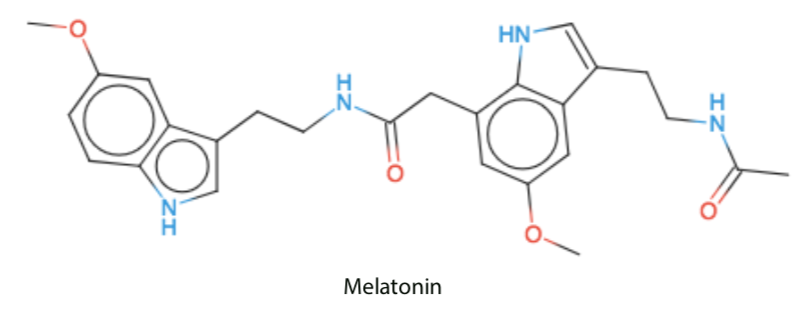
\includegraphics[width=\textwidth]{4fig/sm4.png}
         \caption{Structure of Melatonin}
         \label{fig:st1}
     \end{subfigure}
     \hfill
     \begin{subfigure}[b]{0.495\textwidth}
         \centering
         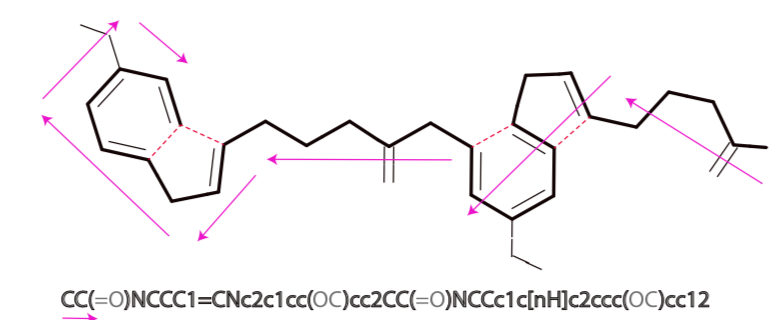
\includegraphics[width=\textwidth]{4fig/sm1.png}
         \caption{Step 1 : Building the C chain backbone.}
         \label{fig:st2}
     \end{subfigure}\\

     \begin{subfigure}[b]{0.495\textwidth}
         \centering
         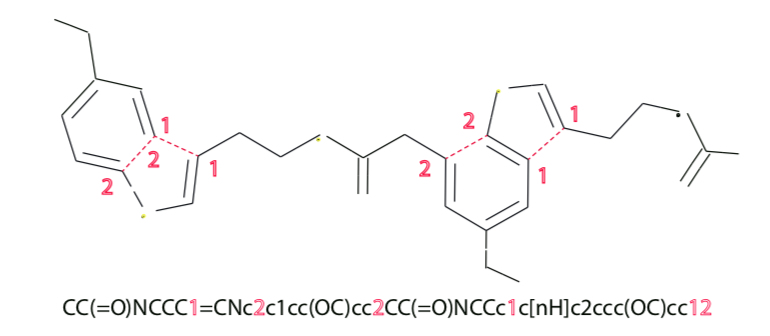
\includegraphics[width=\textwidth]{4fig/sm3.png}
         \caption{Step 2 : Aromatic Rings}
         \label{fig:st3}
     \end{subfigure}
     \hfill
     \begin{subfigure}[b]{0.495\textwidth}
        \centering
            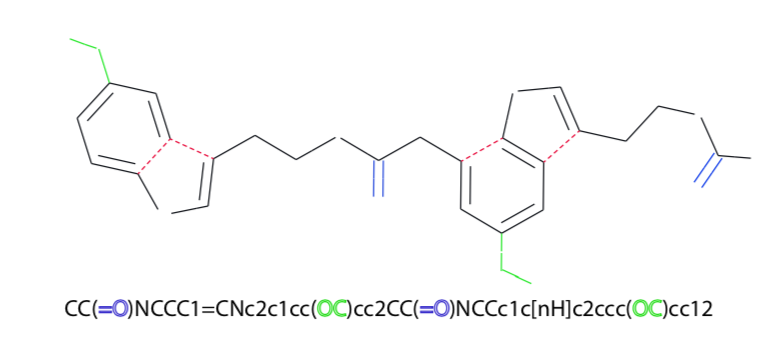
\includegraphics[width=\textwidth]{4fig/sm2.png}
            \caption{Step 3 : Functional Groups }
            \label{fig:st4}
        \end{subfigure}

        \caption{ \textbf{Construction process of a smiles string.} The example compound is Melatonin. Although this does not exist within the atmosphere, it provides a clear example of the smiles string methodology. \autoref{fig:st1} is made using smiles drawer: \citep{smilesdrawer} }
        \label{fig:smiles}
\end{figure}


\subsubsection{Graph Inspired}

\autoref{ch2} - \ref{ch4} have shown the role of graphs in revealing network properties and structure. Graphs in themselves are able to simplify relational data into two/three dimensions for visualisation and algorithmic clustering. Continuing this trend we can represent a species strucuture in the form of a graph (\autoref{sec:specgraph}), as well as converting the structure of a mechanism for dimensionality reduction (\autoref{sec:n2vec})


\paragraph{The species graph (fingerprint)}\label{sec:specgraph}

The structure of a species has long represented using a graph-like layout, \autoref{ch2}. It therefore follows that other methods for representing the graph structure would also apply. One such method is the use of an adjacency (or relational) matrix to describe the relationships between atoms and bonds in a species. Such a methodolgy is already used in the construction of bond and z-matrixes, \citep{mcmgen,zmatrix}. 

The construction of a structure matrix/graph begins with a chemical species. Here the relationships between atoms (\autoref{fig:graphmol}) is converted into an adjacency matrix (\autoref{fig:adjmol}). However since species have different numbers of each atom, a template allowing us to compare different graphs is required. To do this a maximum occurance table (\autoref{table:my_maxoccur}) is created. Here for example BCARY \ch{C15H24}, a sesqueterpine contains the most carbon atoms of any species within the MCM. This universal matrix is now able to contain any possible combination of atoms in a species. 

As machine learning algorithms only vectors as an input, it is possible to decompose the $37^2$ element adjacency matrix into rows, which can then be joined together, Using this method we create a flat array (vector) of 259 elements (518 bytes) which can be used to represent our species.


\begin{figure}[H]
     \centering
     \begin{subfigure}[b]{0.325\textwidth}
         \centering
         \begin{tabular}{c|c}
         \textbf{Atom} & \textbf{Max}\\
         \hline\hline
         &\\
             C & 15 \\
             Cl & 4 \\
             O & 12\\
             N&3\\
             S&1\\
             BR&2\\
         \end{tabular}
          \caption{}
         \label{table:my_maxoccur}
     \end{subfigure}
     \begin{subfigure}[b]{0.325\textwidth}
         \centering
         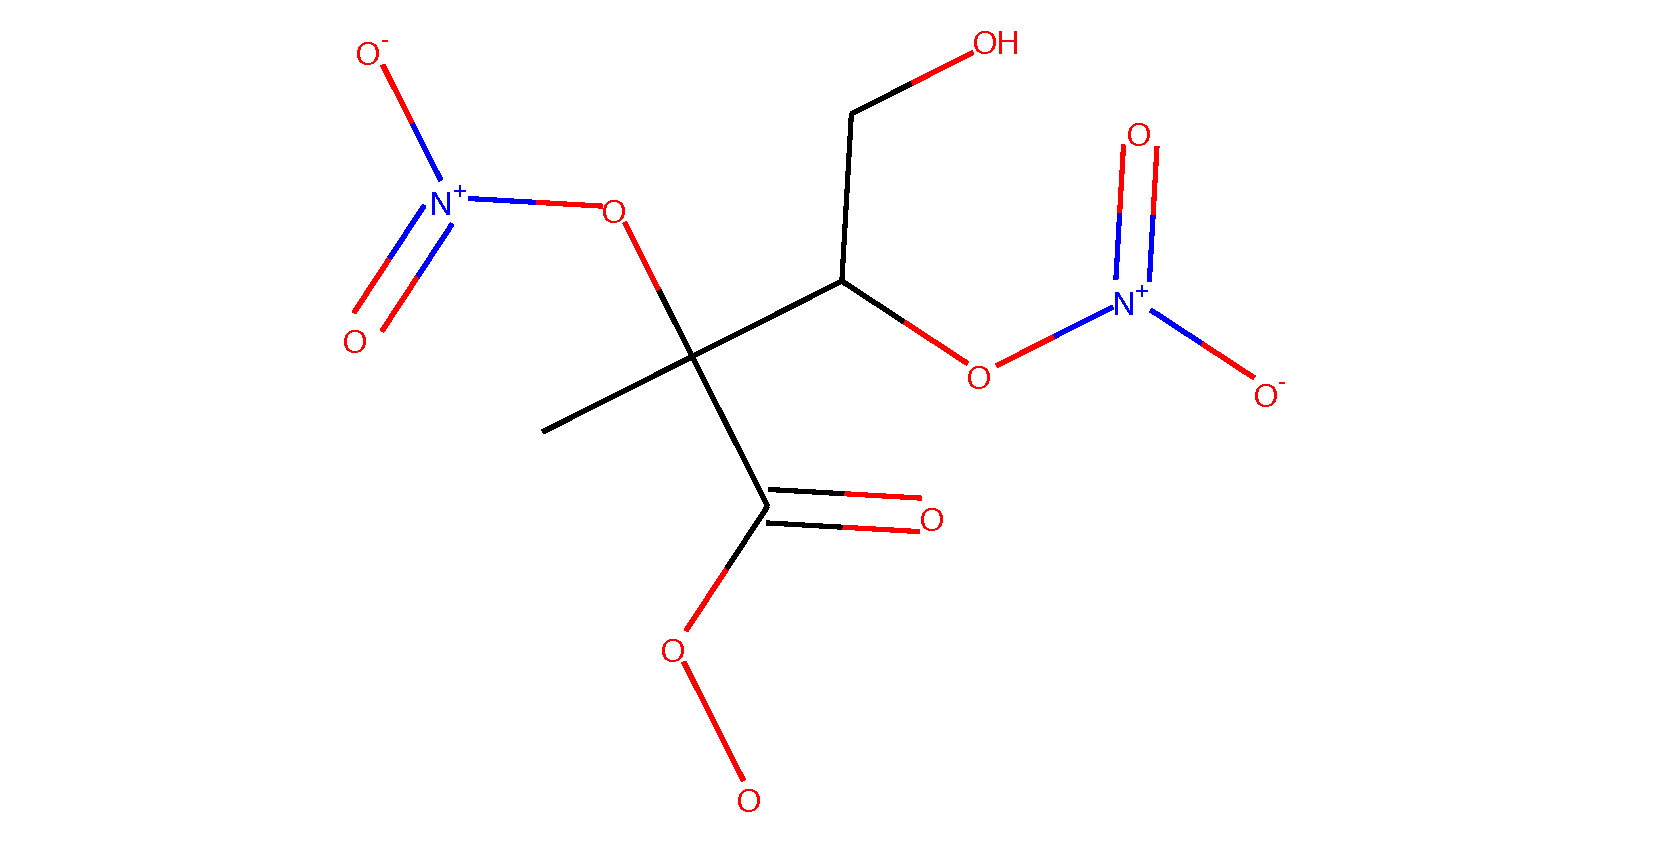
\includegraphics[width=\textwidth,height=.8\textwidth]{4fig/INB1NBCO3.pdf}
         \caption{}
         \label{fig:graphmol}
     \end{subfigure}
     \hfill
     \begin{subfigure}[b]{0.325\textwidth}
         \centering
         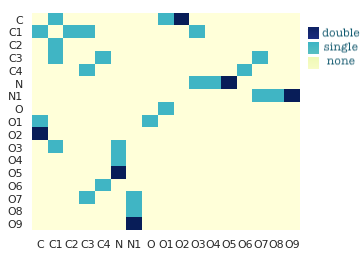
\includegraphics[width=\textwidth,height=.8\textwidth]{4fig/INB1NBCO3_adj.png}
          \caption{}
         \label{fig:adjmol}
     \end{subfigure}

        \caption{ \textbf{Constructing a graph from species structure.} 
        (a) shows the maximum number of times an atom occurs for any single species in the MCM. (b) depicts the graph-like chemical structure of \ce{INB1NBCO3}. This is a highly processed species stemming from Isoprene, and this makes for a good example of the bond matrix. Finally a matrix representing the bonds in \ce{INB1NBCO3} is created from the maximum possible occurance matrix from (a). For simplicity, empty row/column pairs have been removed to produce (c). This matrix will always be symmetrical as the bonds do not have a direction.}
        \label{fig:bondmat}
\end{figure}


\paragraph{Node Embeddings (node2vec)}\label{sec:n2vec}
\autoref{ch2} and \autoref{ch3} showed that the underlying structure of a chemistry mechanism graph contains information about the species and reactions within it. This is seen in \autoref{fig:vk}, where colour represents the ratio of potential oxidation of a species. Here as emitted species become progressively more processed, the number of bonds which may be oxidised deminishes (lighter colours near the centre) until they eventually form carbon dioxide and water. 


\begin{figure}[h]
  \centering
  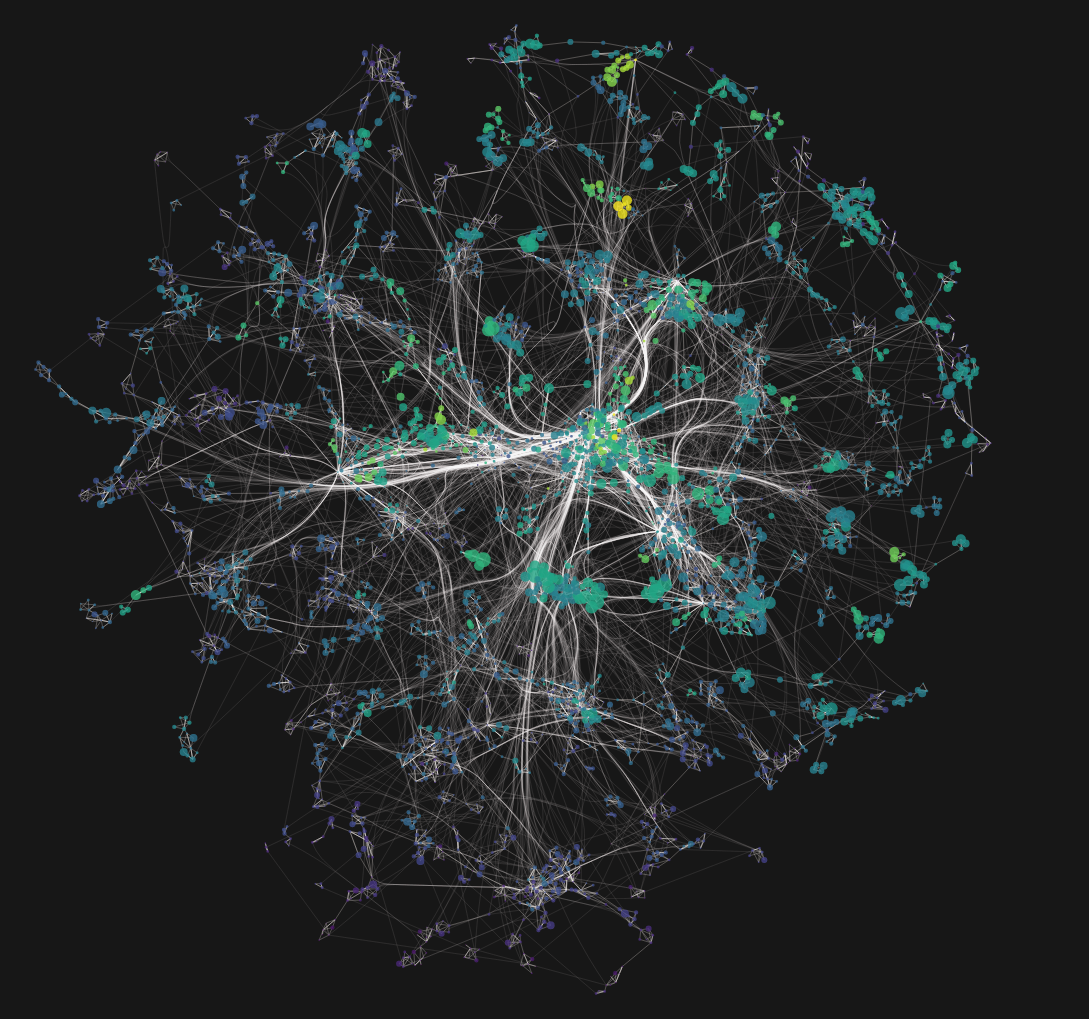
\includegraphics[width=\textwidth]{4fig/graph/oxidised_ratio.png}
  \caption{\textbf{The graph of an MCM subset representing the chemistry within Beijing.} Here colours show the increase of \ce{O-C} ratio as species are oxidised (lighter). All emitted species ultimately tend towards carbon monoxide which is at the centre of the graph. }
  \label{fig:vk}
\end{figure}

This type of strucutral information can be extracted through the use of a natural language processing package capable of transforming a graph into a vector - node2vec \citep{node2vec}. Since this may also be used for dimensionality reduction, it shall be described in the next section (\autoref{sec:n2v}).




\subsubsection{Molecular Fingerprints}\label{sec:fingerprints}


Molecular fingerprints (structural keys) are a way of encoding molecule structure into a queryable series of binary digits. These are predominately used in the filed of chemical-informatics as means of exploring chemical space (a type of property space constructed using pre-determined properties and boundary conditions). Properties are often split into structural and psyico-chemical groups, allowing for the use of data mining techniques in search of molecule similarity (with uses such as the discovery of natural analogues to circumvent side effects and in-tolerances \citep{analog}). Unlike line notations, such as smiles and InChi, molecular fingerprints provide a multi-dimensional classification for chemical species which makes them ideal for machine learning inputs.

\paragraph{Molecular Quantum Numbers (MQN)}
In chemistry the shape, phase and electron occupancy of an atom may be described through the use of four quantum numbers\footnote{These are $n$ principle quantum number, $I$ angular momentum quantum number, $M_i$ magnetic quantum number and $M_s$ spin quantum number.}. The rationalisation of elements based on their structure, and by consequence reactivity, has led to the most iconic tool of the modern-day chemist - the periodic table\footnote{Increasing atomic numbers follow the principal quantum number.} \citep{periodic}. In representing a molecule as a set of 42 quantum numbers, MQN fingerprints produce a multi-dimensional mapping of atom, bond, polarity and topology count \citep{MQN}. Its binary nature not only... application..

[ref fae others... ]

\paragraph{Molecular ACCess System (MACCS)}
MACCS keys are a 164\footnote{Although they are 166-bit keys, there is no real agreement to what the 44th keys' purpose is, and therefore it is often omitted. Within RDKIT this is denoted by a $?$ \citep{rdkitcode}.} bit structural keys formulated through answering a series of structure-related questions. Developed by MDL Information Systems \citep{maccs}, their main purpose lies in being a SMILES Arbitrary Target Specification (SMARTS) system for substructure searching. However their distinct structure key format

makes them highly suitable for similarity detection. In many cases, the optimised version of MACCS keys is cited (\citep{optimised}), although most use cases exploit a variation of the undocumented 166bit keys. We use the implementation presented by \citep{rdkit,rdkitcode} for all molecular fingerprints in this section.


\section{ Dimensionality Reduction Methods}
In the last section we described a number of methods in which the chemical structure of a species could be incoded for direct comparison. However since each input is made up of a multitude of elements, it is still not a simple task determine the differences and similarity between all species in a mechanims. Dimensionality reduction is the process of reducing the number of random variables and only presentind a set of principal values, by mapping a high-dimensional space into a low-dimensional one, \citep{drrandom}. This allows us to flatten a multivariate input into the two dimension required for a simple scatter plot.

In this section we begin by explaining the data preperation required for dimensionality reduction (\autoref{sec:pref}) before desribing the different possible methods of reducing the dimensions of a dataset. 

% 
% Computational algorithms are often described as a black box. This is due to their structure, where we begin with a set of inputs, $X$. These then have a series of operations applied to them, $f(X)$, eventually producing the corresponding output $Y$. In the case of simple linear regression, this intermediate process may be calculated easily by hand. Unfortunately for large datasets, or complex iterative models, this becomes somewhat impractical. Additionally, algorithms such as neural networks or genetic (evolutionary) algorithms may also require the changing of items or hyper-parameters in-situ.
% It is for this reason models need to be evaluated, ensuring that they not only run correctly but register the correct set of features we are interested in.
% 
% For predictive models, an adaptation of the leave-one-out method of assessment is commonly applied. Data is split into a $2/3:1/3$ ratio, whereupon the model is trained on two-thirds of the data, and evaluated in its predictive capabilities on the remaining third. This process is repeated with many permutations of the data to determine an overall model variance. Unfortunately, since we wish to use machine learning (ML) for exploratory data analysis, we need to take a different approach to evaluating the usefulness of a model. Here we take a known property, which through prior knowledge should be highlighted by the models, and compare the output categories output with these.
% 
% 
% \begin{figure}[H]
%   \centering
%   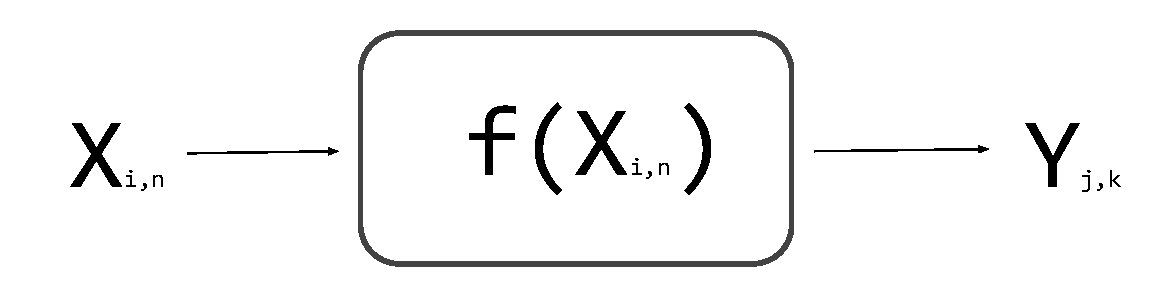
\includegraphics[width=.5\textwidth]{4fig/xy.pdf}
%   \caption{The general flow chart of flow within a machine learnt model.}
%   \label{xy}
% \end{figure}


\subsection{Preperation of the data}\label{sec:prep}
Real-world data is rarely preformatted in such a way that it can be used directly within a computational model. Often values need to be cleaned and corrected to be fit for purpose. In the interest of completeness the two main methods of data adjustment for machine learning are outlined below. These are normalisation and standardisation. 


\subsubsection*{Normalisation}
In the data is without (dimensionless) or of a single unit, it is poissble to rescale the data between a range - most commonly {0,1}. In doing so it is possible to interperate the importance of a value in contrast to the largest recorded value. This gives us a percentage scale spanning the range of the data. Such a range is useful in the definition of colourmaps and describing a values importance relative to the dataset. 
To rescale a dataset we shift the minimum value to zero, then divide by the new maximum of the dataset (Note this is equivalent to the range of the unshifted dataset.)

\begin{equation}
    n(x_i) = \frac{x_i - \min_x }{\max_x - \min_x}
    \label{eqn:n}
\end{equation}



\subsubsection*{Standardisation}
If the components we wish to compare are of differing units, or are expressed with a different scale, normalising them would not produce meaninful data. Instead it is possible to standardise the data by looking at each points deviation from the mean. This is done by dividing the variation of each point from the mean by the standard deviation of $S$ and results in a value between \{-1,1\}, \autoref{eqn:z}. In statistics this is known as the `z-score'\footnote{Possibly because of the American spelling of standardi\textbf{Z}ation?}

\begin{equation}
    z(x_i) = \frac{x_i - \mu_x}{S}
    \label{eqn:z}
\end{equation}\\    


\subsection{Principle Component Analysis}
One of the most well known dimensionality reduction methods is the determination of the principal components through the use of Principal Component Analysis (PCA). PCA works on the assumption that components within a dataset are linear combinations of eachother. By simplifying these linear combinations, it is possible to identify the components which explain the most variability in a dataset - these are the principal components \citep{pca,pca2}.

A simpler interpretation of this would be to adjust the direction of each axis of the data, such that its projection has the largest variability. In doing so it is possible to determine which components contribute the most to changes in the dataset. An example of this is seen in \autoref{fig:2dpca} where the second component of the original data may be removed with little effect on the overall result of the data. Such methods have applications in compression and signal filtering [REF REF]


\begin{figure}[h]
    \centering
    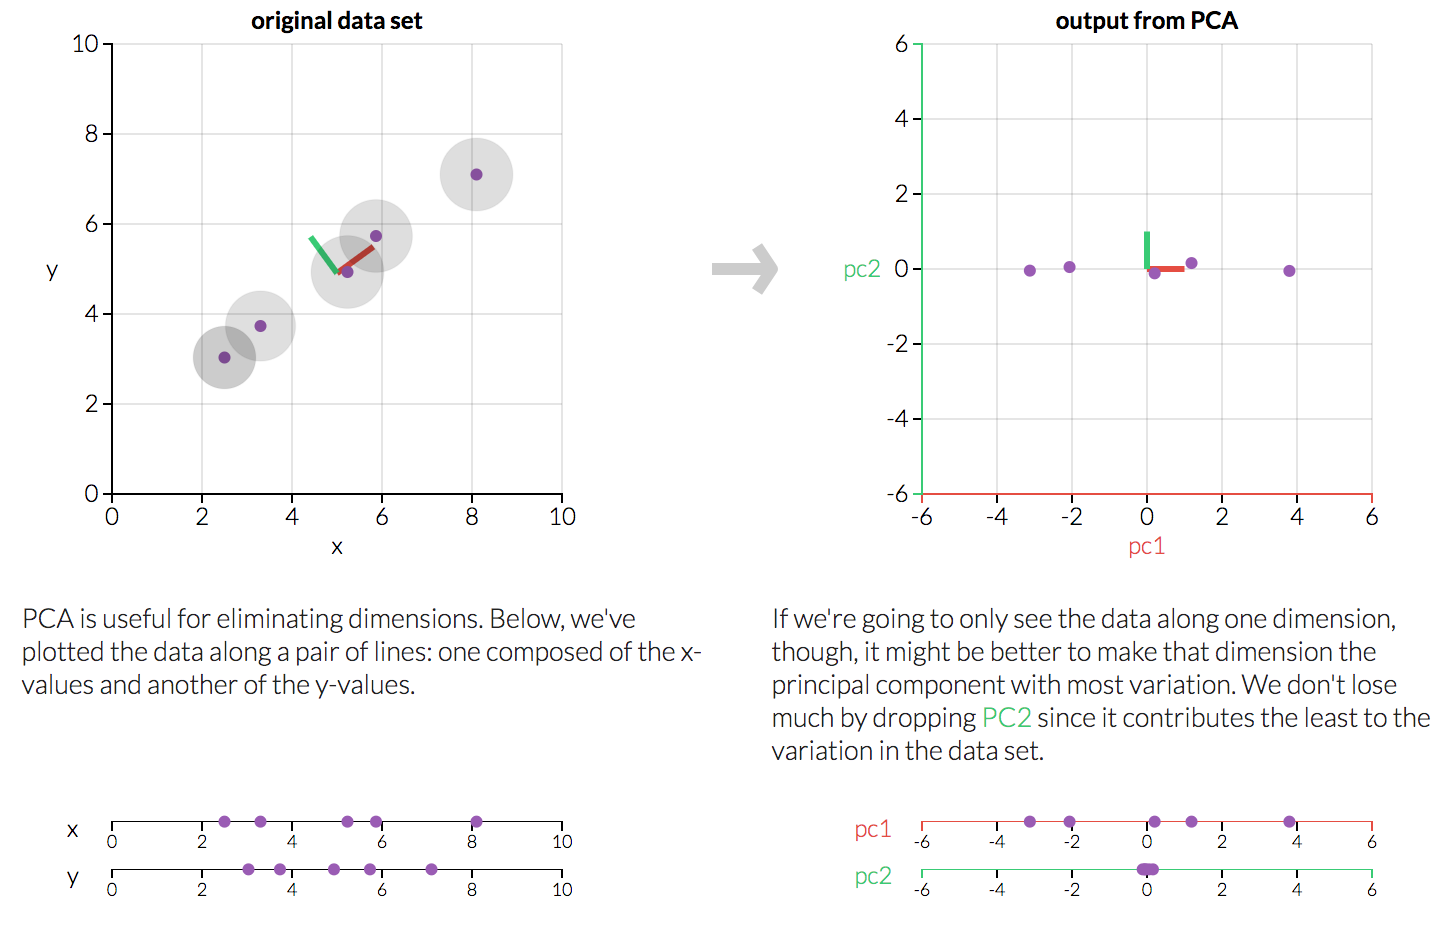
\includegraphics[width=.8\textwidth]{./4fig/pca2d.png}
    \caption{\textbf{Determining the Principal Compnent of a sample dataset.} It can be seen that in a change in axis to follow the first principal component (right), it is possible to explain most of the variation in the samle dataset (left). Source: \citep{pcaim}}
    \label{fig:2dpca}
\end{figure}


\subsubsection{Mathematical explanation of PCA}
\emph{\textbf{Note:} The basic statistics/mathematics required to understand this section is shown in \autoref{apendix:pca}. Please read this if you are not familiar with any of the terms below.
}

The mathematics behind PCA consists of first calculating the covariance matrix. This is an $n \times n$ matrix outlining how strongly each variable changes with every other. Using this we can calculate both the eigenvalues and eigenvectors of the matrix \footnote{These need to be unit vectors, although most packages already do this out of the box.}. This may be done using a computational package such as numpy or scipy \citep{numpy,scipy}.

We can now sort the eigenvector columns by influence using their eigenvalues. This way a feature data-set can be produced by removing vectors of low influence. The final feature dataset can now be transposed and multiplied by the transpose of the original dataset. This produces an output dataset containing each principal component of the desired dimension.



\subsection{t-Distributed Stochastic Neighbor Embedding (t-SNE)}

t-SNE is an algorithm designed with visualisation in mind \citep{tsne}. Rather than representing the data through a series of linear transformations, t-SNE uses local relationships to create a low-dimensional mapping, much in the same way as a fully connected force graph, \autoref{fig:tsneforcegraph}. This allows the ability to capture non-linear structures in the data which cannot be done through linear mapping methods (e.g. PCA).

The algorithm itself can be broken down into two parts[REF ttsne introduction paper]:
\begin{itemize}
  \item [1.] Create a probability distribution which dictates relationships between neighbouring points
  \item [2.] Recreate a lower-dimensional space following the probability distribution established in 1.
\end{itemize}

The main reason t-SNE produces good results is that it can handle the `crowding problem' very well.


\subparagraph{Crowding Problem}\label{sec:overcrowd}
The crowding problem is a product of the `curse of dimensionality. This is because, in high dimensional space, the surface of a sphere will grow much quicker than one in a lower dimension space. This means higher dimension spaces will have more points at a medium distance from a certain point, \autoref{fig:dimcurse}. When we map our data into a lower dimension, data will try to gather at its medium distance, resulting in a more `squashed', and thus crowded, output.



\begin{figure}[H]
  \centering
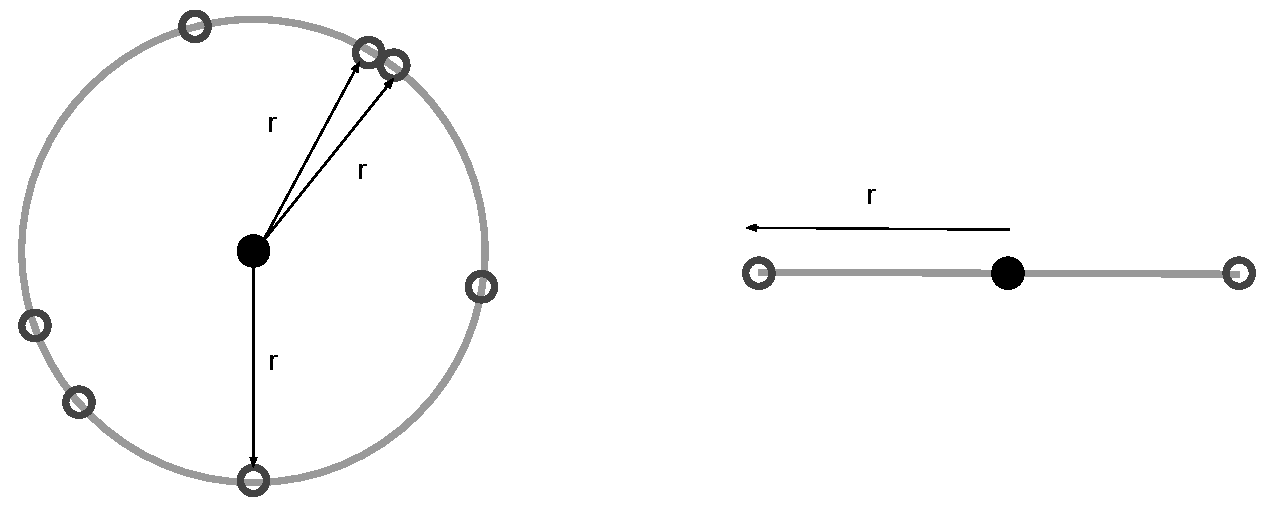
\includegraphics[width=.5\textwidth]{4fig/dimcurse.pdf}
\caption{An example of how the curse of dimensionality affects the mapping of points a certian distance from eachother. }\label{fig:dimcurse}
\end{figure}




\subsubsection{Mathematical explanation of t-SNE}
%https://mlexplained.com/2018/09/14/paper-dissected-visualizing-data-using-t-sne-explained/

%
% The general process is given by the etymological dissection of the acronym, with `t'  standing for the student T probability distribution and S, N (stochastic and neighbour) explaining the use of the distribution across neighbouring points in space.

In the original paper \citep{tsne}, the algorithm is described using the etymologic dissection of its name.

\paragraph{Step 1}
First we begin with Stochastic Neigbour Embedding (SNE) - the distribution across neignbouring datapoints in our high dimension space. This is done by converting the high dimensional Euclidian distances between points into conditional probabilities representing their similarity:

\begin{equation}
p_{ij} = \frac{\exp(-\left \| x_i - x_j \right \|^2 / 2\sigma_i^2)}{\sum_{k \neq l} \exp(- \left \| x_k - x_l \right \|^2 / 2\sigma_i^2)}
\end{equation}

Here $p_{i|j}$ is the conditional probability that $x_i$ may pick $x_j$ as a neigbour. This is proportional to the probability density of a Gaussian $\sigma_i$ centered at $x_i$.

\subparagraph{Perplexity}
Since we want the number of neighbours of each point to be similar in number and prevent a single point from having a disproportionate influence on the entire system we introduce a hyperparameter named \emph{perplexity}. This works by ensuring that $\sigma_i$ is small for points in densely populated areas and large for spare ones. This means that the perplexity of a system can be thought of as a scale of the number of neighbours considered for any one point. Generally, values between 5 and 50 are considered to give good results, with larger perplexities taking global features into account, and by consequence smaller ones, local features.

\paragraph{Step 2}
Now a probability distribution describing the relationship between points has been formulated, we wish to express this as a low dimensional mapping of our inputs $X$ in terms of our output dimensions $Y$. Naturally, we would want to make the low dimensional mapping represent a similar (Gaussian) distribution as in Step 1. However, it often causes issues presented by the `overcrowding problem'\autoref{sec:overcrowd}. This is because the gaussian has a `short tail', and thus nearby points are likely to be pushed together. A solution to this is the student t-distribution which has a longer tail \footnote{The distribution employed is a t-distribution with only one degree of freedom. This is identical to the Cauchy distribution}:

\begin{equation}
q_{i|j} =\frac{(1 + \left \| y_i - y_j \right \|^2 )^{-1}}{\sum_{k \neq l} (1 + \left \| y_k - y_l \right \|^2 )^{-1} }
\end{equation}

\emph{\textbf{Note:} The definition and explination of the Student t-distribution is given in \autoref{apendix:tsne}.
}

The optimisation of this equation can be achieved through the use of \emph{gradient decent}\footnote{\textbf{Gradient Decent}
This is an optimisation algorithm used to minimise a function by iteratively moving in the direction of the steepest descent. This can be used to find local minima and is defined by the negative of the gradient. Its primary usage in machine learning is the updating of parameters (coefficients in linear regression and weight in neural networks).}
 on the Kullback-Leibler divergence \autoref{appendix:kl} between distributions $p$ and $q$. Here the gradient is used to apply an attractive and repulsive force on the items\footnote{A positive gradient signifies attraction, whilst a negative one corresponds to repulsion.}.




\subsection{PCA vs t-SNE, a quick comparison.}

PCA is one of the most used DR algorithms[ ref list ]. It is fast, simple and easy to use and very intuitive. The PCA algorithm works by creating a lower-dimensional embedding which best preserves the overall variance of the dataset. Clusters created from the algorithm are grouped in ways, such that they preserve the greatest variance.

The main drawback of PCA is that it is a linear projection. If our data happened to be in a `swiss roll' (spiral) pattern, we would not be able to `unroll' it. This is because PCA works by viewing the data from different perspectives, much like casting a shadow from various directions. With such an example, there is no one way we can do this that unfurls the spiral.

t-SNE, on the other hand, is a relatively new method [ref 06/08 paper]. Its greatest asset is that it is not limited by linear projections. Although more computationally intensive for large datasets, t-SNE produces visibly cleaner results. Unlike in PCA, t-SNE cannot be trained on additional data at a later point, however, the output clusters are more visually distinct (they have less overlap). Much like in a force graph, the output from t-SNE is scale-invariant. This means that whilst the location of clusters in a PCA reduced representation have an attributable quality, those produced by t-SNE will not necessarily contain the same information.

To test the differences between the two methods, a box model run representative of the chemistry within Beijing was used. The aim was to classify the diurnal profiles of each species concentration. To do this we standardised all the results and extracted the third day from a spun up model. These results were then fed into both the PCA and t-SNE algorithm. \autoref{fig:threegraphs} show the differences between the models. In \autoref{fig:pcac} we can see that the embedding is prone to overlap between species, with sample groupings (non-yellow species)\footnote{Species with similar profiles were grouped,\autoref{fig:tco} } often being densely stacked on top of each other and indistinguishable from collections of species around them. Although only a slight improvement for the specified dataset, the t-SNE reduction allows the points to be better distributed, improving the definition of the group boundaries.

\begin{figure}[H]
     \centering
     \begin{subfigure}[b]{0.495\textwidth}
         \centering
         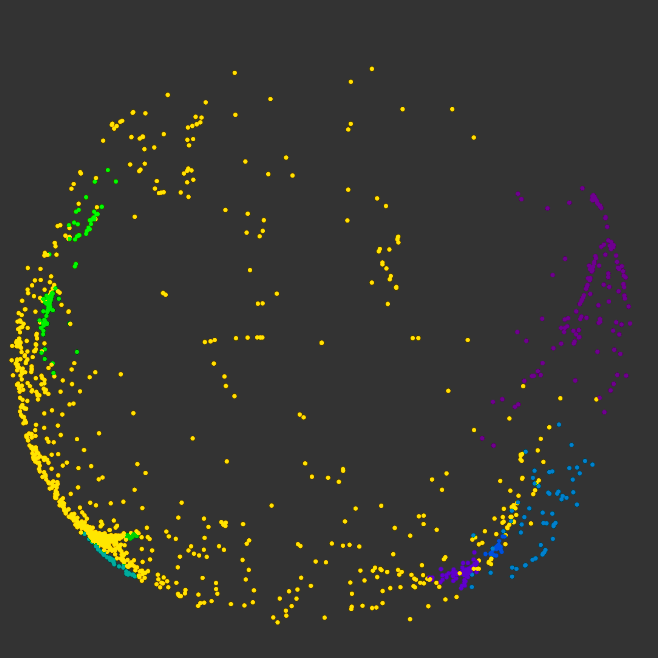
\includegraphics[width=\textwidth]{4fig/ppca.png}
         \caption{PCA}
         \label{fig:pcac}
     \end{subfigure}
     \hfill
     \begin{subfigure}[b]{0.495\textwidth}
         \centering
         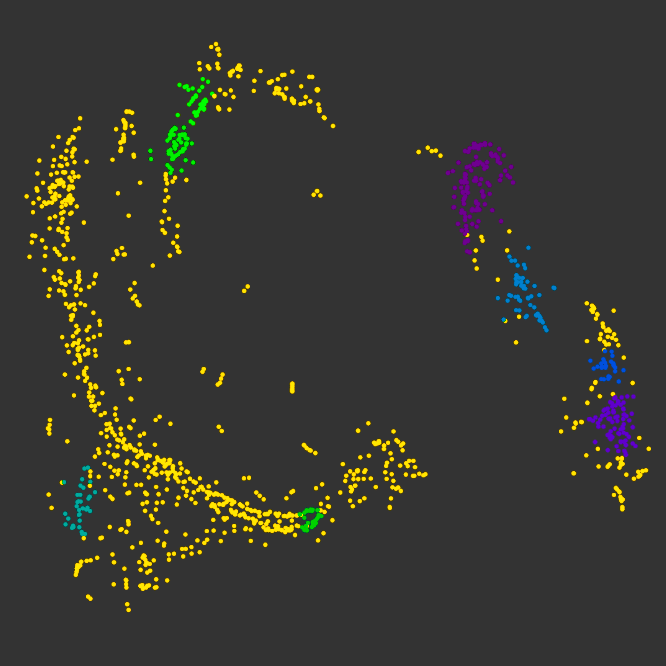
\includegraphics[width=\textwidth]{4fig/ptsne.png}
         \caption{t-SNE}
         \label{fig:tsnec}
     \end{subfigure}
     \hfill \hfill
     \begin{subfigure}[b]{\textwidth}
         \centering
         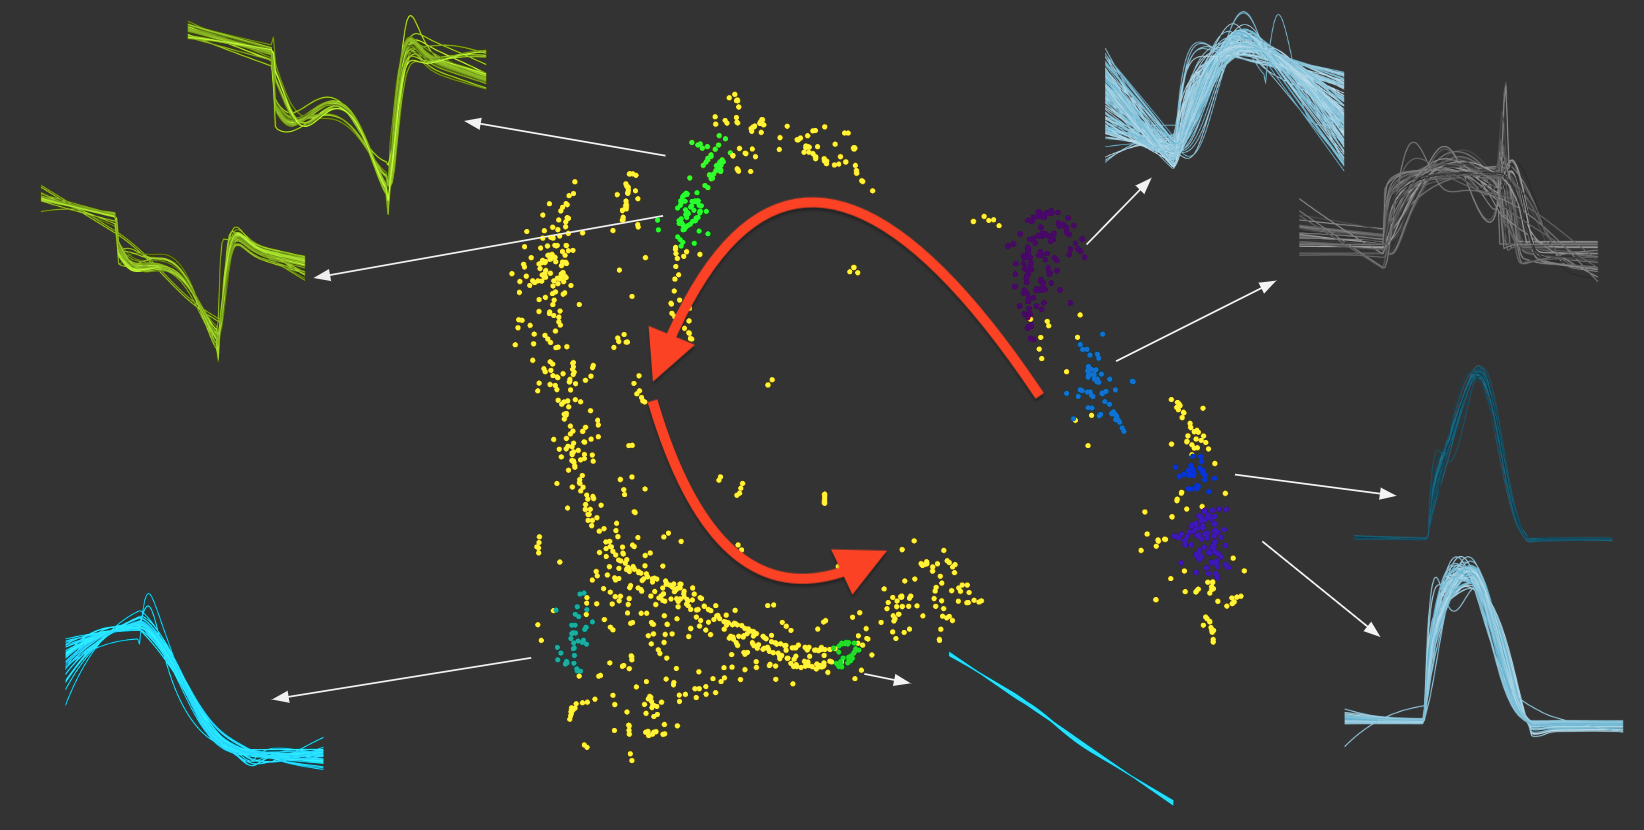
\includegraphics[width=\textwidth]{4fig/ptsneall.png}
         \caption{t-SNE with cluster outlines.}
         \label{fig:tco}
     \end{subfigure}
        \caption{Three simple graphs}
        \label{fig:threegraphs}
\end{figure}




\subsection{The Auto-Encoder (AE)}
Auto-encoders are a subclass of neural networks which are primarily used for dimensionality reduction. Rather than predicting a numerical output autoencoders focus on the construction and deconstruction of data through the use of an encoder and decoder pair. The encoder takes an n-dimensional input and applies a compression, reducing it to the number of dimensions in the bottleneck layer. This reduced dataset is then reconstructed within the decoder. Such a process not only allows for an easy understanding of the error of the reduced data but can also be used in the filtration of noisy or pixelated data [ref].\\


\begin{figure}[H]
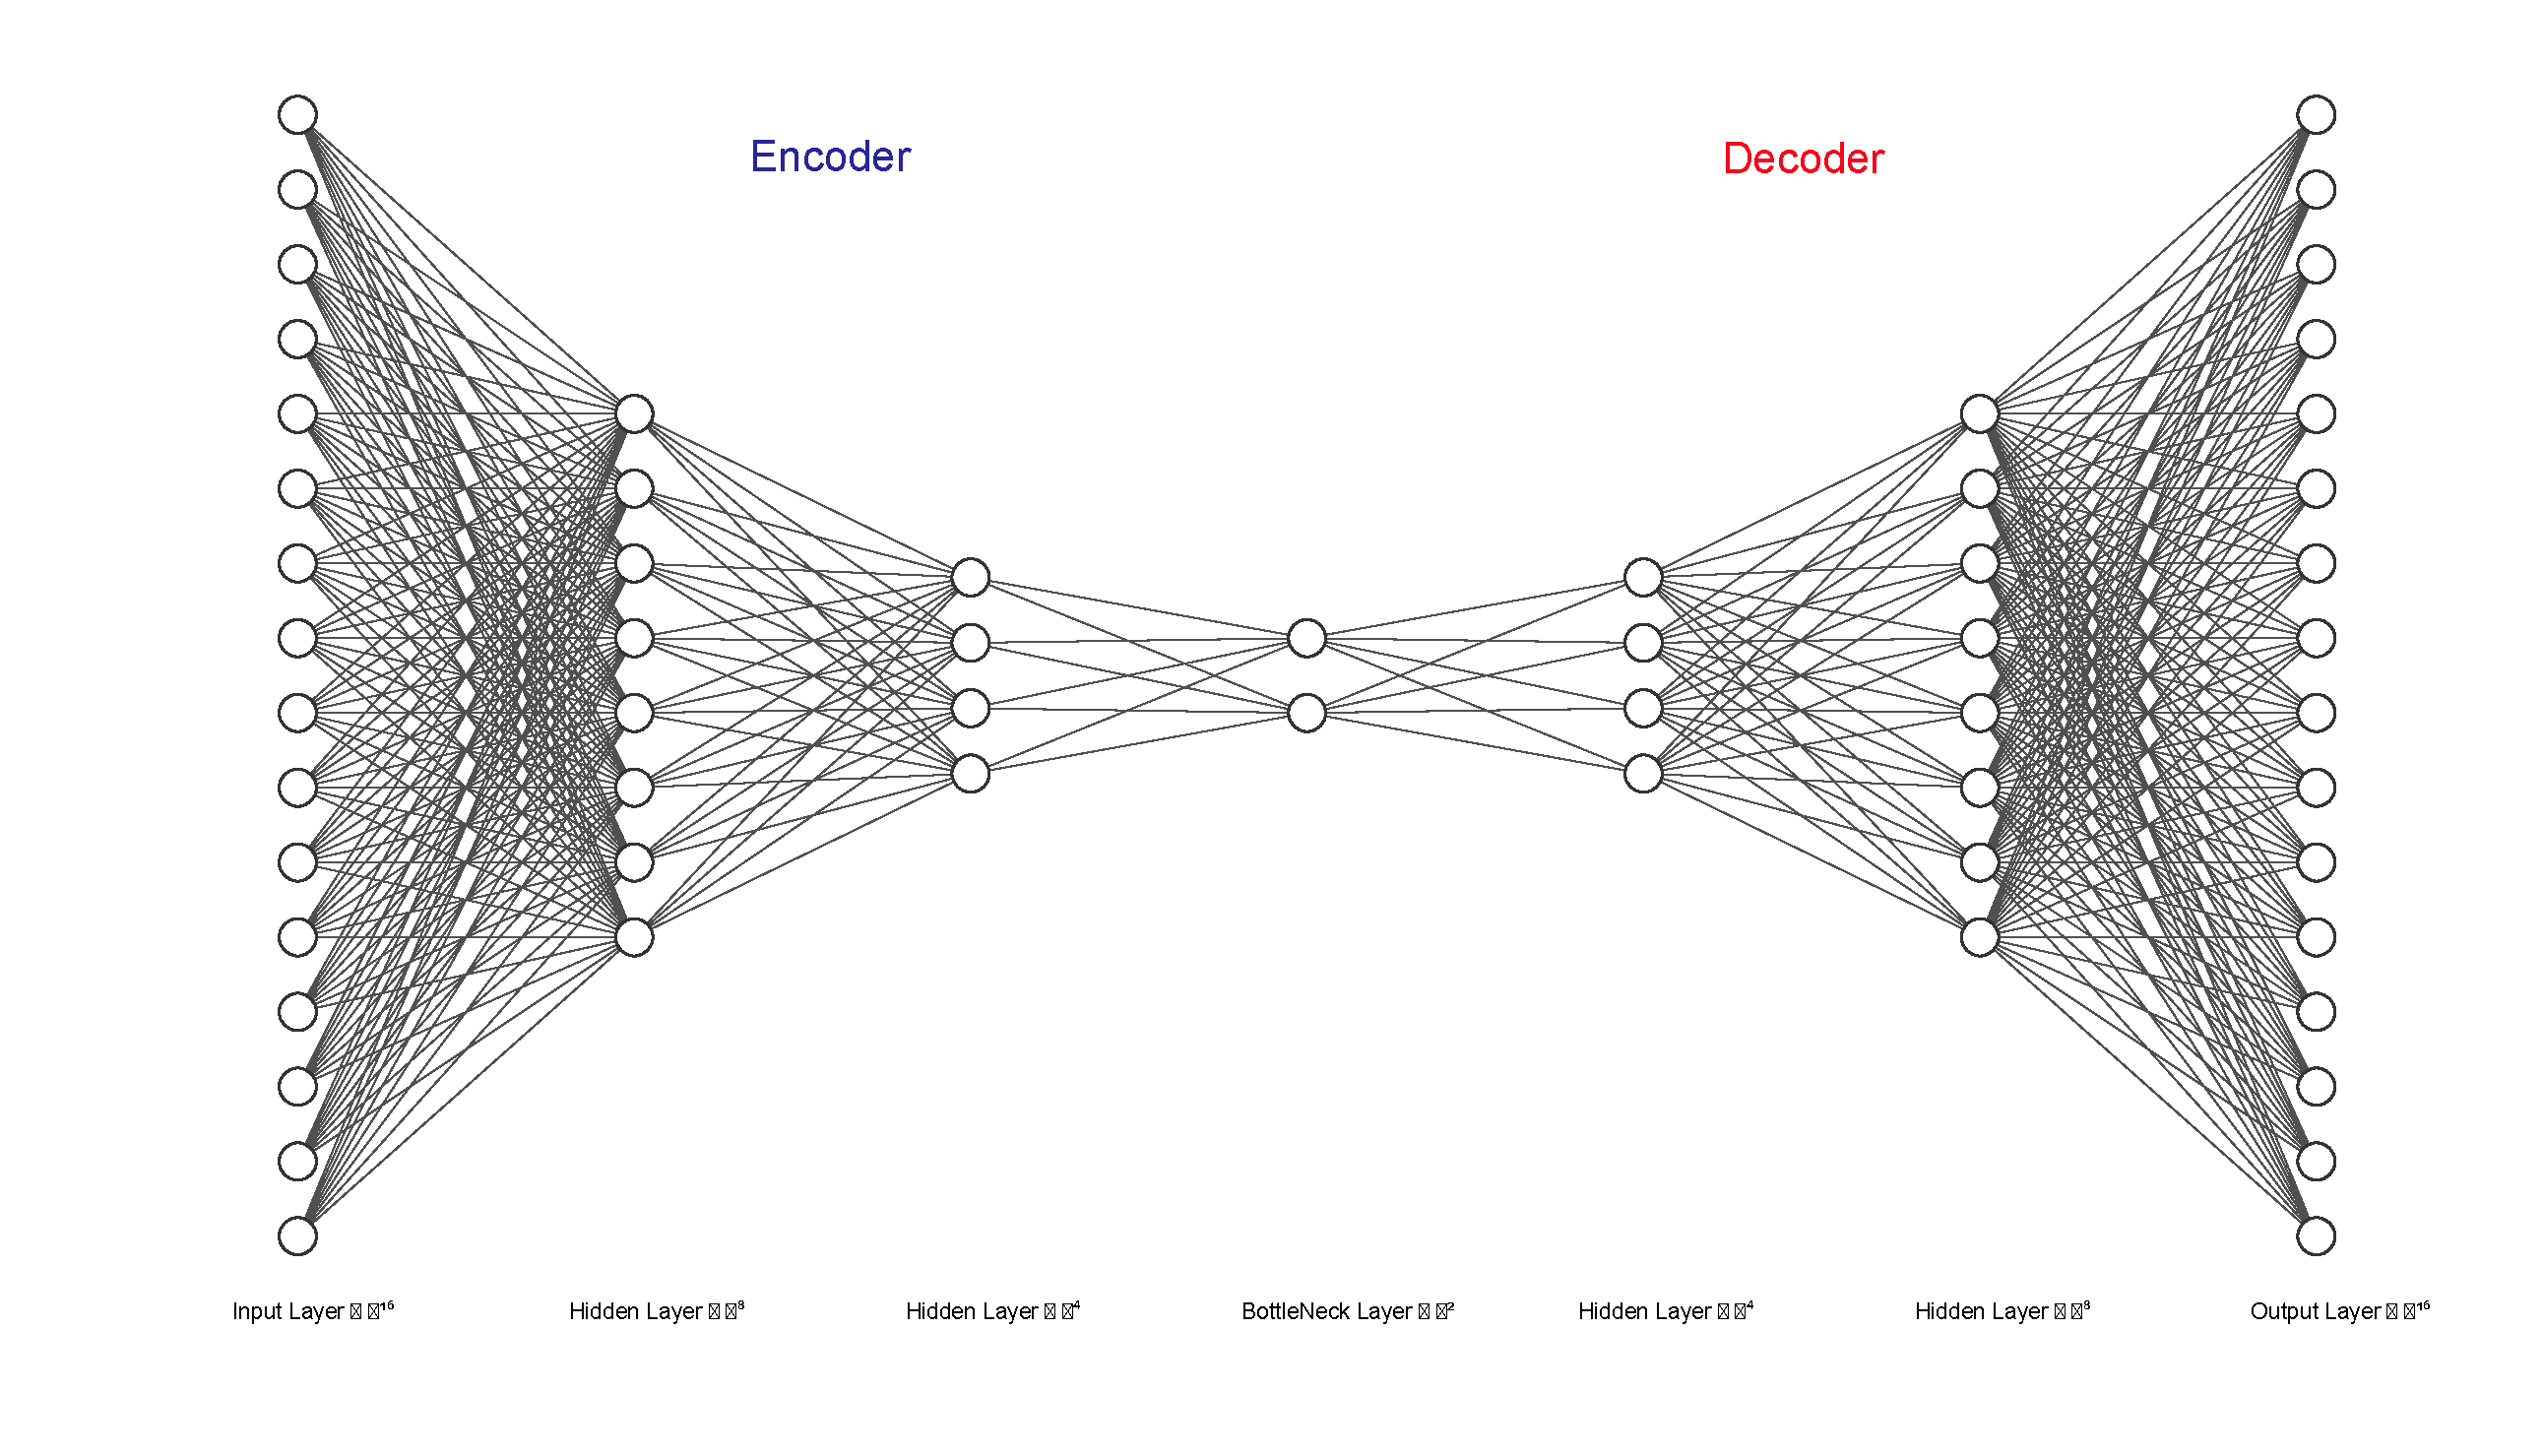
\includegraphics[width=\textwidth]{4fig/ae.pdf}
\caption{An example autoencoder structure which reduces a 16 dimentional input to 2. Draw with the aid of \citep{drawae}}
\end{figure}


Usage in image reconstruction, signal processing or feeding large data into other models. \\

There are two features of an autoencoder that make it powerful. The first is the ability to sample your latent space using the decoder. This means we can establish features that correspond to gaps between our data points - which can have its application if the data used is sparse or incomplete. Next comes the inherent non-linearity of the model. As an autoencoder is just a neural network, the amount of information passed through each link between layers is governed by an activation function. Should this activation function be linear, the reduced dimension will be much akin to a PCA decomposition. However unlike PCA, in reducing the number of dimensions, we do not discard any data, but rather combine it - as per the nature of the links of the network. In trying to model/fit non-linearity, we have a range of activation functions to choose from. These are:



\subsubsection{Demonstration of non-linear activation functions}

To demonstrate the effect of these we take a sample isopleth of Methane and Ozone, reduce it to two dimensions, and then reconstruct it. Here we can see that some of the non-linearity of the original dataset has been lost when discarding the third principal component during PCA. Using a tanh activation function in an auto-encoder however, recreates much of the original properties of the data.


\begin{figure}[H]

\begin{subfigure}{.33\textwidth}
  \centering
  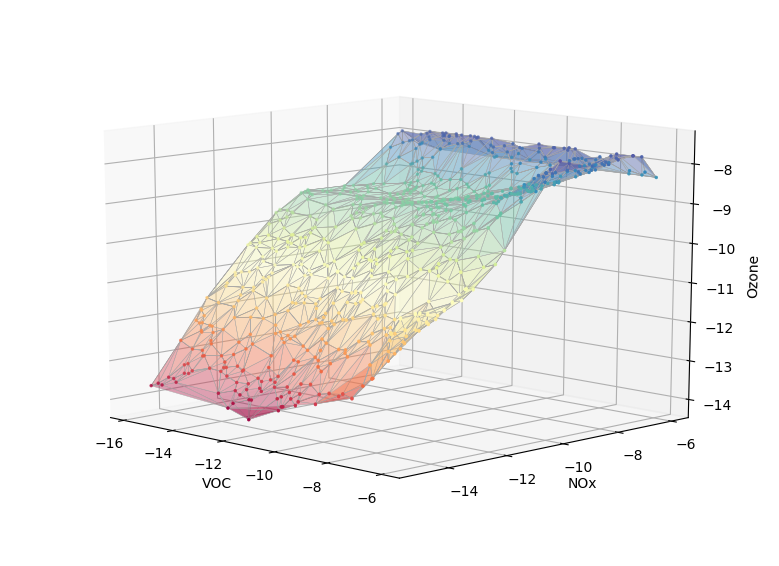
\includegraphics[width=\textwidth]{4fig/original.png}
  \label{fig:orig}
  \caption{Original}
\end{subfigure}%
\begin{subfigure}{.33\textwidth}
  \centering
  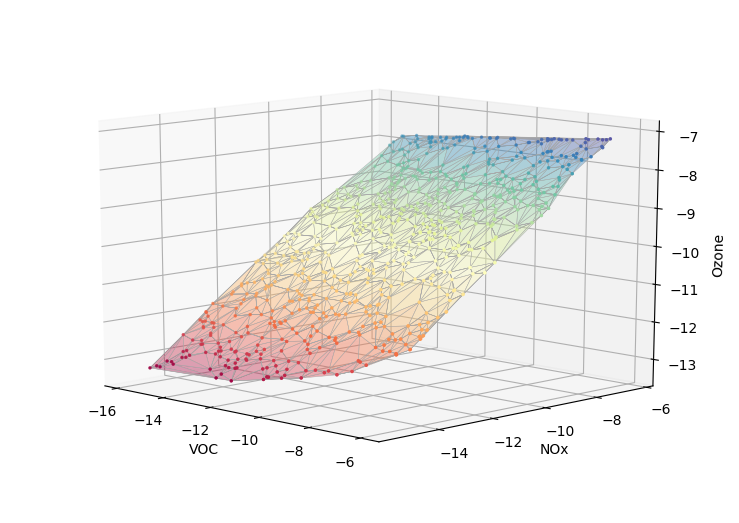
\includegraphics[width=\textwidth]{4fig/rpca.png}
  \label{fig:pca}
  \caption{PCA}
\end{subfigure}%
\begin{subfigure}{.33\textwidth}
  \centering
  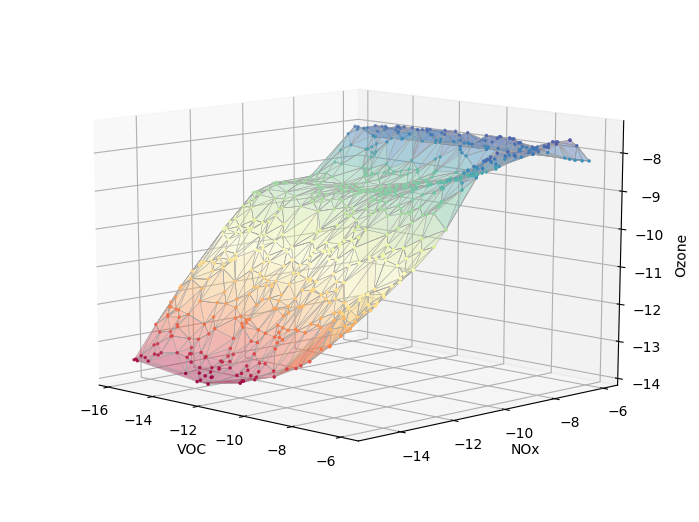
\includegraphics[width=\textwidth]{4fig/rae.png}
  \label{fig:ae}
  \caption{AE (Tanh)}
\end{subfigure}%


\caption{Reducing the original dataset by 1 dimension and reconstructing it using different methods. Figure created using 300 simulations initialised with NOx (variable), Methane (variable) and Ozone (constant) using a Latin hypercube. The results are then plotted and converted into a surface using Delaunay triangulation. }
\end{figure}

%
% \subsection{Graph Auto-Encoders (GAE)}
%
% It was seen that graphs neural networks (GNN) were far more powerful in 2016...
% Training time and results\\
%
% Graph auto-encoders are an extension to these, applying the auto-encoder structure to a GNN. Here we may feed information about the relationships between items in our network, as well as the features representing them.
%
% This method of representation has its purpose in both classification and link prediction. In terms of an autoencoder, we may use this to extract the graph embeddings at a lower dimension. In \citep{karatAE} it is shown that GAEs are able to extract an embedding of the graph communities within a network. In other papers, GAEs have been used for matrix completion, and in-turn link prediction \citep{gaelink}. This makes them a potentially powerful tool in the visualisation, understanding and prediction of atmospheric chemical graphs.


\subsection{Node2Vec}\label{sec:n2v}
 Node2Vec is an embedding algorithm designed to generate vector representations of the nodes in an \textit{undirected} and \textit{unweighted} network. This not only allows the input of graph derived relationships into other models, but can also be more computationally efficient, by circumventing the need for expensive composition, whilst producing better predictions on some network-related tasks compared to more classical methods, such as PCA \citep{node2vec}.


\begin{figure}[H]
  \centering
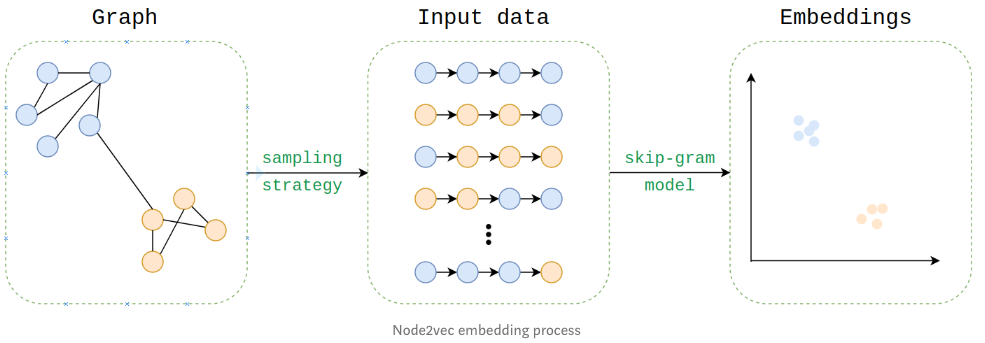
\includegraphics[width=\textwidth]{4fig/n2vproc.png}
\caption{The process of converting a graph into a vector using Node2Vec. Source:\citep{n2vimg}}\label{fig:n2vprocess}
\end{figure}


The process of converting the graph structure (\autoref{fig:n2vprocess}) into a numerical vector node embedding starts by taking a series of $2^{nd}$ order random walks. These describe the neighbourhood of a node in the form of a set of random walk paths, much in the same way words are dependant on their neighbours within a sentence: \autoref{eqn:w2varrow}.


\begin{equation}
ISOPRENE \rightarrow OH \rightarrow TISOPA \rightarrow ISOPBO_2 \rightarrow TISOPA \rightarrow...
\label{eqn:w2varrow}
\end{equation}


\subsubsection{Input / Sampling}
The probability and path depend both on a set of arguments and a random seed provided to the model. The return and input parameters $p,q$ determine how fast we explore the network and our probability to leave the neighbourhood, \autoref{fig:n2vedge}. In a network, where the previous path is from $t$ to $v$, we may calculate the probability of returning to $t$ as $1/p$, going to a mutual node connected between $t$ and $v$ as 1, and viewing a new node as $1/q$.
If $q>1$ we have a high probability to end up at nodes close to $t$, and with $q<1$ we are likely to explore other nodes. Additionally if we chose $p> \max{q,1}$ we are less likely to return to an already visited node ($p < \min{q,1}$ is likely to generate a backwards step). Since we wish to generate a `local' view, but do not wish to return to $t$ we select  $q \ge 1$ and $p > q$ our parameters as  $p = 2.0,q=1.1$.  In the case of a weighted graph (something that we are \textit{not} exploring within this chapter) the resultant $alpha$ value calculated is further multiplied by the edge weight.

To run the simulation we use the python 2 code provided by the original paper \citep{node2vec} with a set of 50000 random walks, each of length 9. The reasoning behind this is that we have a large graph, with a power-law like structure (within only a couple of steps we are connected to every other species within the network - that is if we do not include the inorganics, which in this case we are).

\textit{NOTE: This process takes over a week to compute, and then the binary file containing all walks in character form approaches 10 GB, for the complete MCM. ...in serial... }

\begin{figure}[H]
  \centering
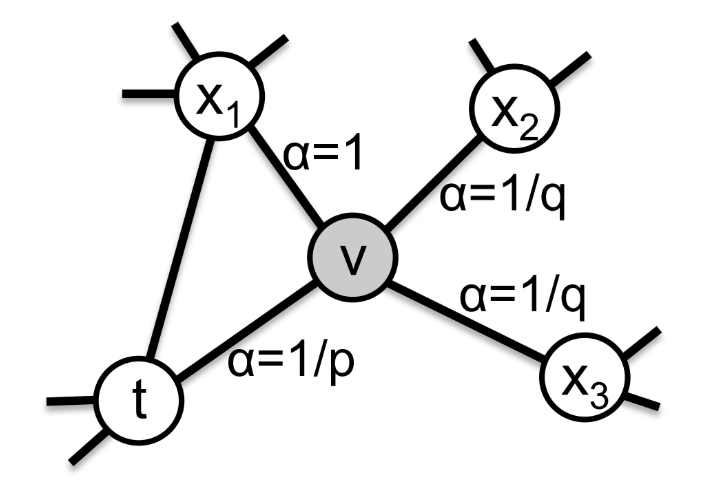
\includegraphics[width=0.5\textwidth]{4fig/n2vedge.png}
\caption{Calculation of the random walk path. Source:\citep{node2vec}}\label{fig:n2vedge}
\end{figure}

\subsubsection{Word2Vec}
Once we have constructed our random path `sentences', we can make use of the well renowned word2vec algorithm developed by Google \citep{w2v}. The word2vec algorithm is similar to an auto-encoder in many regards, but rather than learning word embeddings through reconstruction, it looks at the words (or species in our case) which neighbour each other in our corpus. This form of representation has found many uses beyond the realm of natural language processing. Some of these are objects, people, code, tiles,genes and graphs \citep{objects,people,code,tile,gene,graph2vec}.



https://skymind.ai/wiki/word2vec
http://mccormickml.com/2016/04/19/word2vec-tutorial-the-skip-gram-model/




\section{Visualisation of clustering}\label{sec:drvis}

In assessing the validity of clustered space, we require a level of exploratory data analysis. To reveal features of interest we plot the reduced 2D dataset and apply interactivity coupled with a selection of visualisation techniques described below. This section outlines the different visualisation methods which have been used.

\subsection{Viewing the 2D species embeddings}
Since the different DR algorithms return data on various scales, comparison between the outputs is not straightforward. To overcome this all outputs in both the $x$ and $y$ directions are normalised (scaled between \{0,1\}), before being plotted as a scatterplot. 


\subsection{Exposing overlapping data}
To be able to interactivity highlight data, a user must first be able to select it. This proved difficult if many of the nodes of a tight-knit cluster are overlapping. As an initial test, node sizes may be reduced, to check if this solves the problem, however, this may often leave points smaller than is possible to easily select. The other solution which was used is to create a force-directed graph where each point is strongly attracted to their initial position. Here we can apply collision detection, whilst still preserving the overall grouping of nodes within a cluster - a technique that was seen in \autoref{ch4}.


\subsection{Gooey Effect (Gaussian Blur)}
Taking a quote from \cite{lessmore}:
\emph{``The more stuff in it, the busier the work of art, the worse it is. More is less. Less is more. %The eye is a menace to clear sight. 
''} and combining it with the work from \autoref{ch1}, we realise that showing each species, when observing overall clusters just add unnecessary clutter to the images. Instead, since we are only interested in the clusters as a unit, a `gooey effect' filter can be applied. This works by merging nearby points into a single water-like blob using a gaussian blur\footnote{Here a gaussian blur of standard deviation 3.7 and a colour matrix [1 0 0 0 0  0 1 0 0 0  0 0 1 0 0  0 0 0 37 -5] is used.}. Here since each point is allocated a colour, if a colour gradient exists, then there are multiple clusters occupying the same place. The aim of this is to reduce the cognitive load on the end-user by reducing the number of distinct objects that they need to take in.



\subsection{Four Colours Theorem}\label{sec:4col}
When plotted, the number of clusters detected often exceeds the number of categorical colours available. In cartography, it has been noted that the colouring of neighbouring polygons should at most take 4 colours. This is the origin of the four colours theorem, \cite{fourcolour}, of which a greedy implementation has been applied.

The aim of this is to show item boundaries (for instance countries, or in our case clusters), whilst reducing ambiguity (if say two neighbours have the same colour). The algorithm I adapted uses the Delaunay tesselation scripts contained within DataDrivenDocuments.js (d3js) \cite{d3js}. This partitions our plane into polygon-regions with boundaries at the furthest distance from each point (Voronoi cells) \cite{delaunay}. First, we chose a random cell and assign it a colour. 
Next, all its neighbours are recursively iterated, giving them the lowest possible colour in a list, which does not match any of their neighbours. Although such a greedy approach does not produce an optimum result it allows for the colouring of data with $\le 5$ distinct colours, as is shown in \autoref{fig:4col}.


\begin{figure}[H]
  \centering
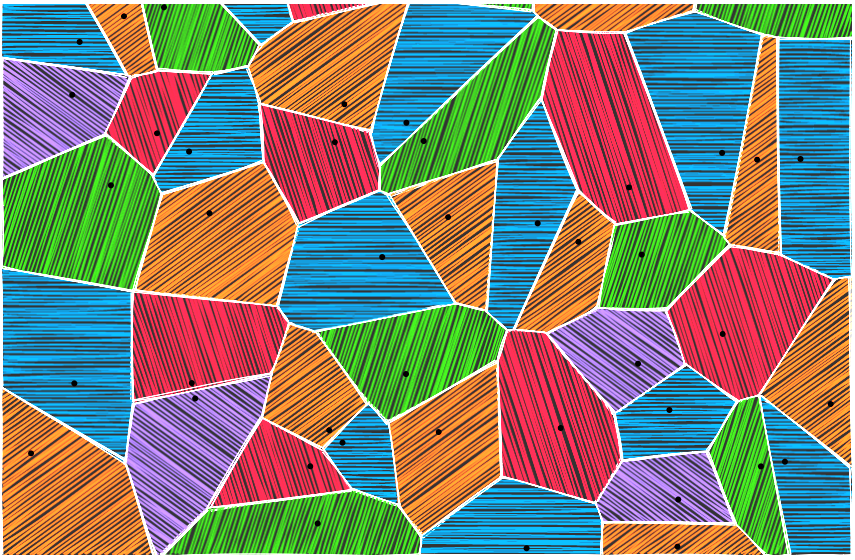
\includegraphics[width=.8\textwidth]{4fig/4col.png}
\caption{\textbf{An example 4 colour matching} This uses the first implementation of the algorithm mentioned in \autoref{sec:4col}. The greedy approach does not often find the optimum solution, which may result in 5 colours instead. Observable Notebook : \cite{4colobs}}\label{fig:4col}
\end{figure}


Having defined all the visualisation techniques we move on to explain the clustering algorithms which are used, and how `goodness of fit' may be measured in the clustering context.

%%%%%%%%%%%%%%%%%%%
%%%%%%%%%%%%%%%%%%%











\section{Cluster Evaluation}
The previous section discussed methods of visualising the reduced data for use with interactive exploratory data analysis. In this section we look at the use of vector clustering algorithms\footnote{Vector clustering is the grouping of data based on their proximity or density to other nearby points} (\autoref{sec:drclustt}) to highlight groups in a 2D dataset, as well an automated method of assessing the quality of the clusters selected (\autoref{sec:silo}) and feature extraction (\autoref{sec:drfeature}).



\subsection{Automated selection of clusters}\label{sec:drclustt}
    When it comes to clustering data points in a dataset, there exist a range of methods which may accomplish a task, \autoref{fig:clustereval}. Most often the k-means, \citep{kmeans}, is used as it is fast and simple to understand. However, its linear method of partitioning cannot capture the splits between non-linear relationships of real data. The other problem is that an estimate for the number of expected clusters is required - something that is often unknown without prior understanding of the data. When this is the case often it is easier to manually select the nodes with interactivity.

In contrast, density-based clustering techniques such as GMM (\citep{scikit}) or DBSCAN (\citep{DBSCAN}) tend to be better at locating non-linear trends in the data. The DBSCAN algorithm asses the distribution of data across a certain location. This allows clusters with a high density of datapoints to be located without the need for a predefined number of clusters. Another method: OPTICS (Ordering Points To Identify the Clustering Structure), \citep{optics}, shall be used\footnote{ If using Python 2, the library for this needs to be extracted from the sci-kit-learn library for python 3 package and altered to run with the previous version. (See copy in attached code.)}. This is an adaptation of the DBSCAN algorithm which does not require the specification of a minimum distance between points (for the density estimate)- instead, we specify a gradient for the distribution and the minimum number of points for a cluster to be classified.


\begin{figure}[H]
     \centering

         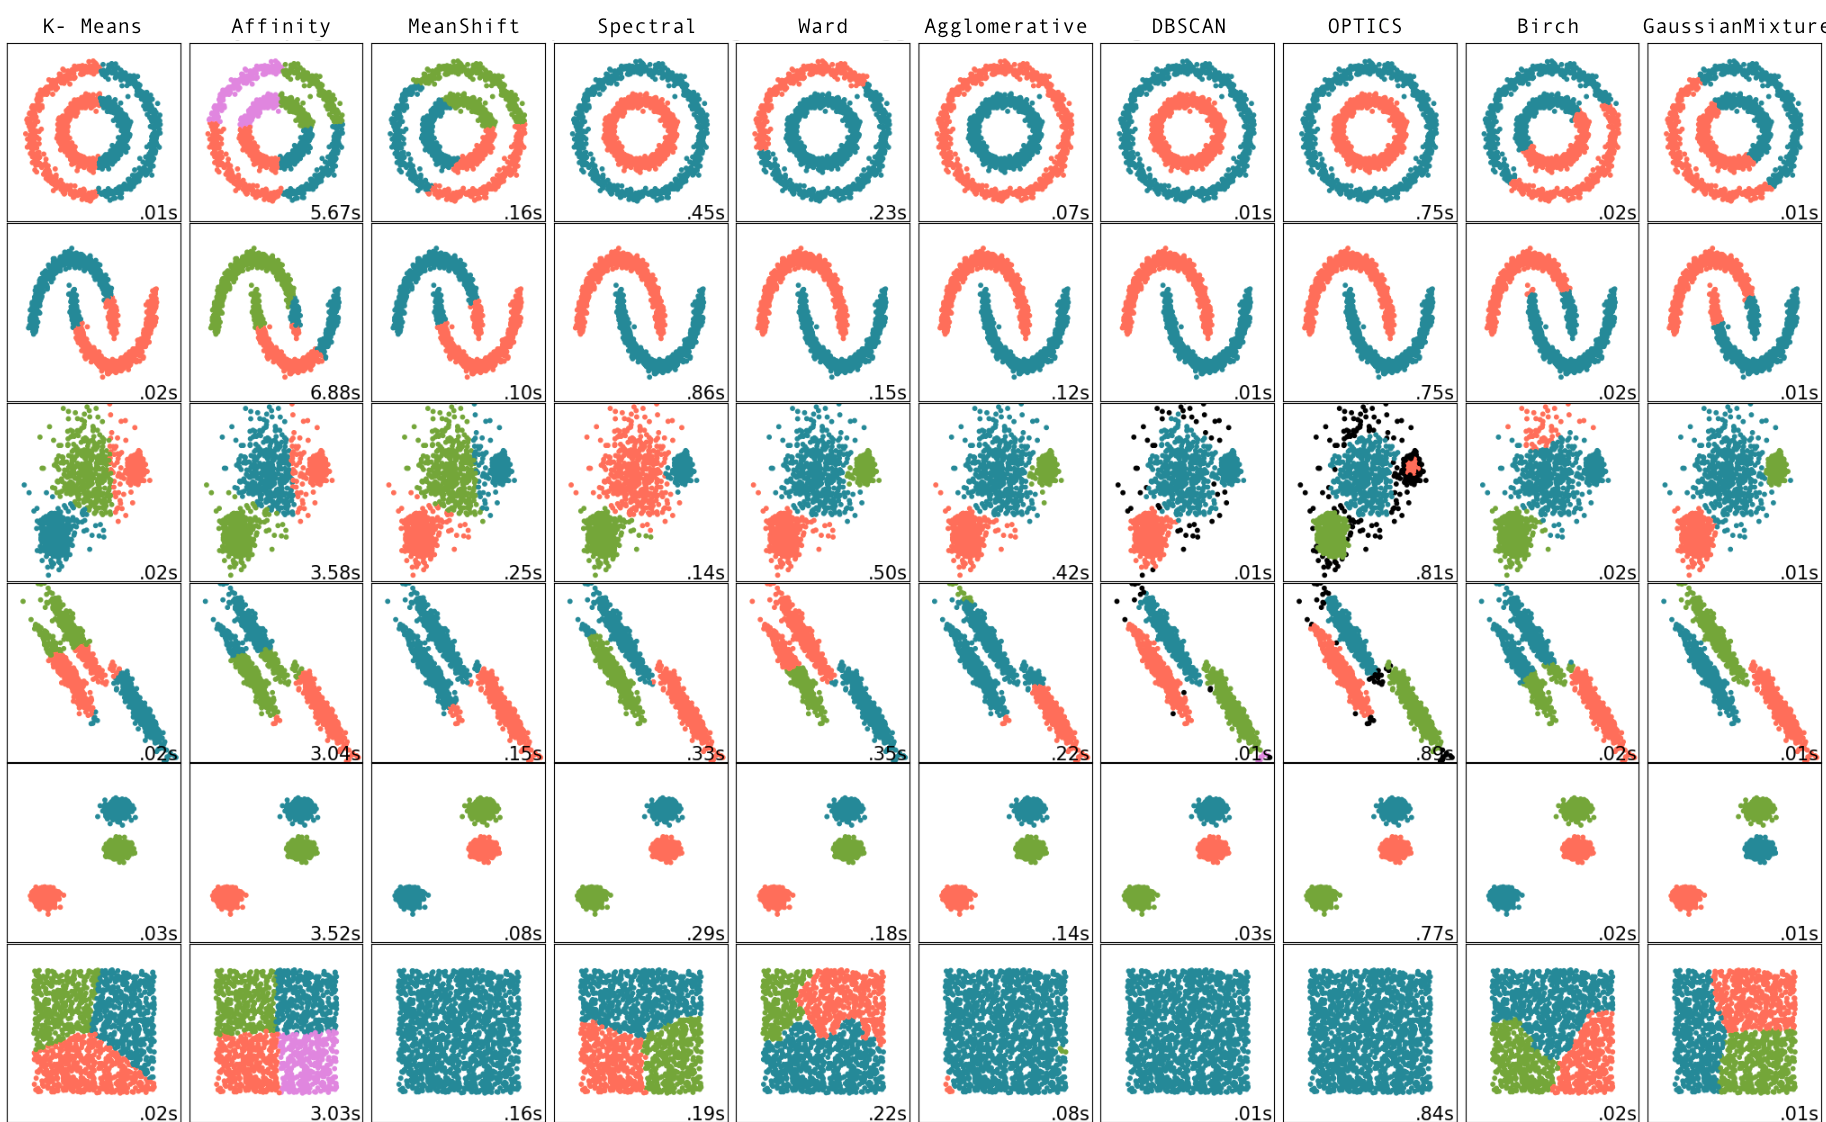
\includegraphics[width=\textwidth]{4fig/clustereval.png}

        \caption{\textbf{A comparison of different clustering methods on a toy dataset.} The plot shows the performance of several vector clustering algorithms in Scikit-Learn. Cluster algorithms are represented across the horizontal axis and several types of datasets are across the vertical. Clustered groups are coloured. Source: \cite{clustereval}}
        \label{fig:clustereval}
\end{figure}


When deciding which algorithms to use, each algorithms' ability to partition non-linear data is considered. 
The first two rows of \autoref{fig:clustereval} show data which cannot be partitioned linearly, here spectral, DBSCAN and optics are the only clustering algorithms to identify both correctly. It is for this reason that we shall look at these for the remainder of the chapter. 

In selecting a value for the results section, several clustering algorithms, with a wide range of input parameters are run. From these, the values with the best silhouette coefficient (\autoref{sec:silo}) are taken. 




\subsubsection{Clustering (Silhouette) coefficient}\label{sec:silo}
The silhouette measure is a tool used for acessing the validity of a set of clusters. Here each cluster is represented as a silhouette, based on the comparison of its tightness and separation. To calculate the silhoette coefficient we look at the intra-cluster $a$ and the mean inter-cluster\footnote{Inside and between different clusters.} distance $b$. The silhouette cluster can then be described using \ref{silhouette,sklearn}:

\begin{equation}
s(i) = \frac{b(i)-a(i)}{\max{ a(i), b(i)}}
\end{equation}

This gives a value $-1 \le s(i) \le 1$. Values near zero suggest overlapping clusters, 1 - dense, well-separated clusters and negative values indicate that a sample may have been incorrectly classified. In using this method we can get an overview of how well individual objects lie within their assigned cluster.




\subsection{Feature Extraction}\label{sec:drfeature}
Upon establishing a set of DR datasets, and their groups (the clusters of species they contain), it is important to evaluate what input features they represent. Rather than doing this manually we make use of Random Forests. 

\subsubsection{Random Forrests}
Random forests, \citep{rfrr}, are a subset of ML algorithms called ensemble learning. This means that they train a large number of decision trees, each on a random subset of the original features. A decision tree is a tree formed from a series of conditionals\footnote{Questions with a True/False answer}, much like a perceptron network (\autoref{sec:perceptron}) with binary activation functions. Random forests introduce a level of additional randomness by selecting only a subset on which to create each decision tree. This may introduce a higher bias, but lowers the overall model variance which creates a better (more robust) model. Such methods have been applied to replacing the computationally expensive process of chemistry integration of GEOS-Chem (a global 3D model of tropospheric chemistry) \citep{geosrf} and the prediction of global sea-surface iodine based on observations coupled with sea-surface temperature, depth, and salinity, \citep{iodene}.

\subsubsection{Calculating importance using Random Forrests}
Since random forests are in essence a collection of decision trees, it is possible to generate a `decision tree aggregate' to visualise the ensemble structure of the random forest, \citep{forrester} (\autoref{fig:iodenetree}). Alternatively, if all that is required is the relative importance of each feature, the RandomForrestClassifier from \cite{sklearn} provides a quick and easy way of understanding which features matter, 
\citep{handsonml}. This works by aggregating the weighted nodes which use a certain feature using the number of samples and then scales the result to 1. We use this method to access the overall importance of features within each DR output and identify the differences between clusters.
%bagging an aggregate collection of TreeS


\begin{figure}[H]
     \centering
         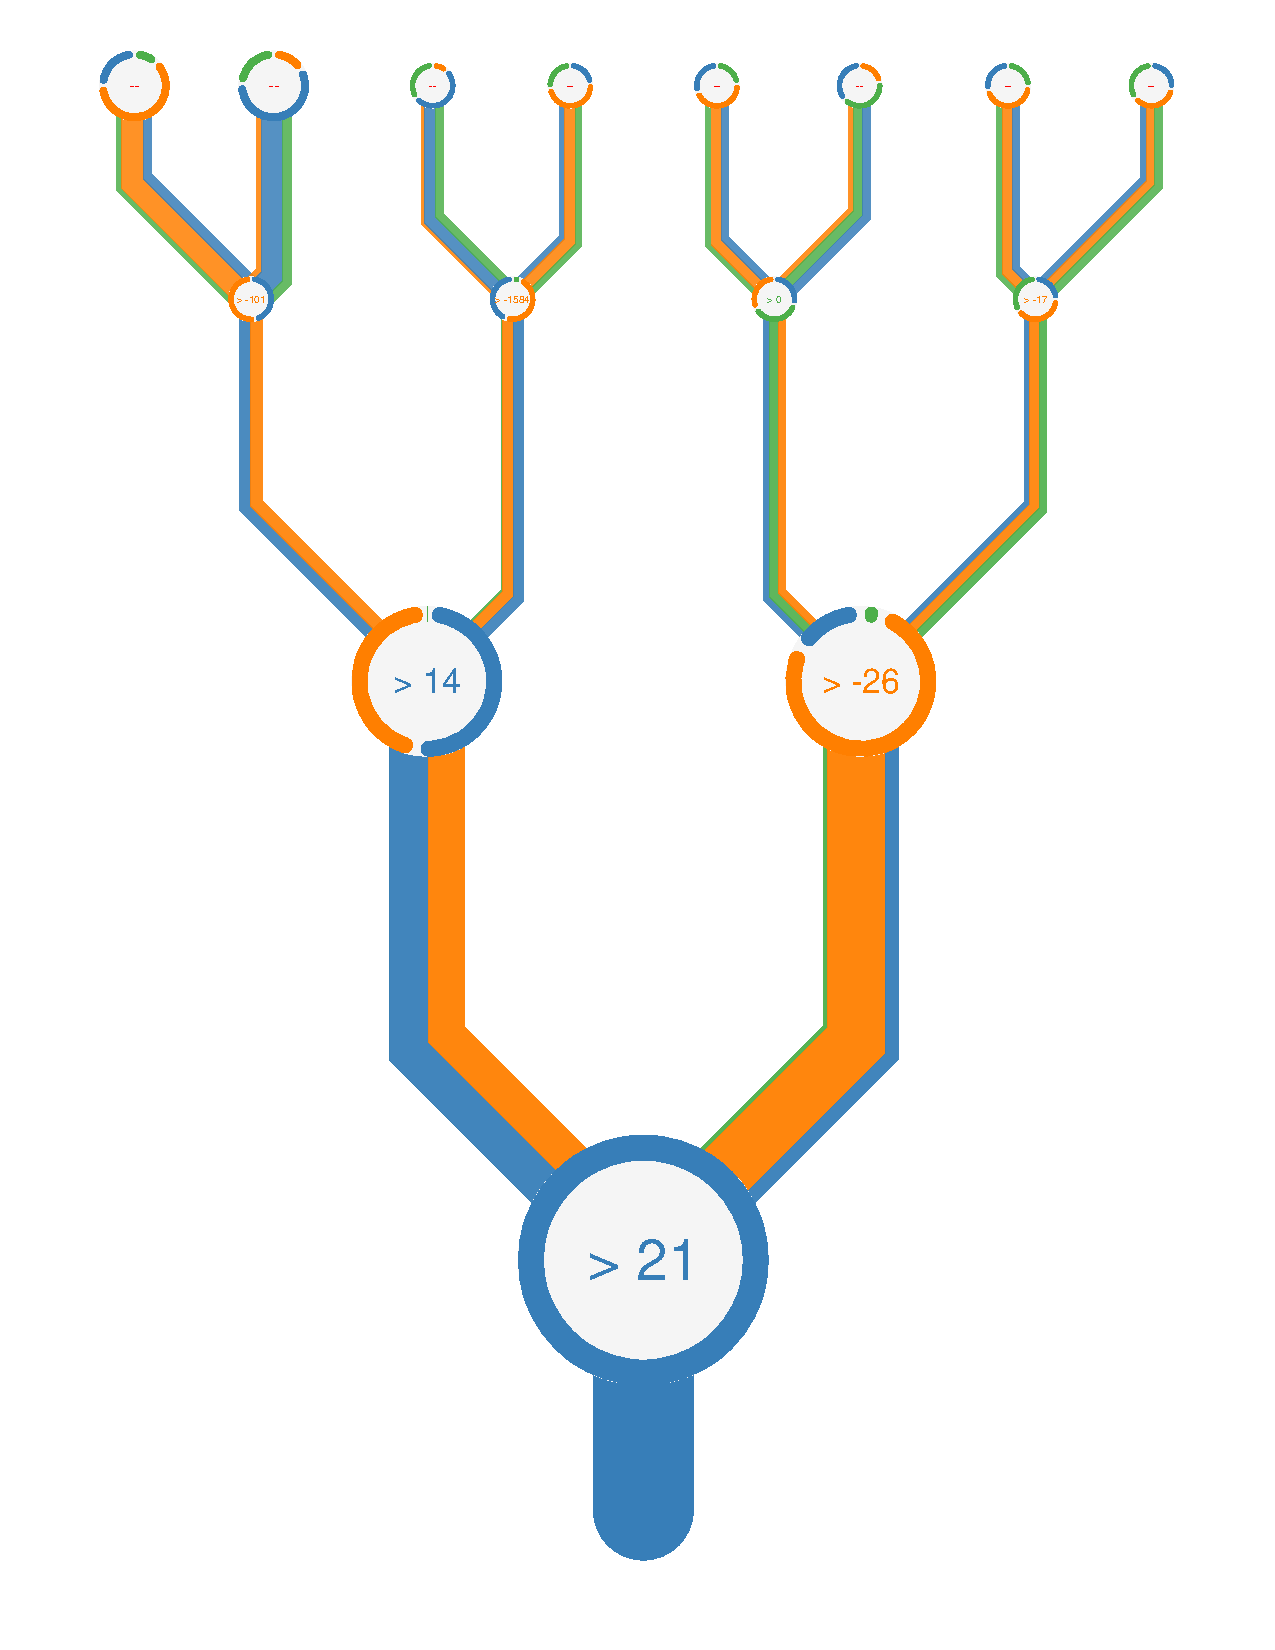
\includegraphics[width=.55\textwidth]{4fig/Oi_prj_features_of_RFR(TEMP+DEPTH+ChlrA)_for_depth_5_white.pdf}
        \caption{\textbf{A decision tree aggrogate from a random forrest plotted with the Epiphyte version of the TreeSurgeon program \citep{forrester}.} The data originates from \cite{iodene} and the imporance of Tempearature (blue), Depth (orange) and Chlorophyll $a$ (green).}
        \label{fig:iodenetree}
\end{figure}


% 
% Random Forrest Classifier from sklearn, top n features.
% https://github.com/MaartenGr/CustomerSegmentation/blob/master/Customer%20Segmentation.ipynb
% https://www.ncbi.nlm.nih.gov/pmc/articles/PMC5732374/

\textit{NOTE: The only downside is that Random Forrests are in themselves ML techniques which also need to be evaluated. To do this, as they are simply being used as indicators of cluster properties which we are to explore further, we can initiate a collection of 300 random Forrest classifiers, from which we take the median.}







\section{Results}
% 
% There exist many methods to define the chemical structure of the species within the MCM. In this section we shall attempt to evaluate their effectiveness for exhibiting the defining functional groups and charactaristics used for constructing the mechanism. In order to do this, we shall use a range of linear and non-linear DR techneques as a means of clustering the data. 

\subsection{CLuster distribution}

Start with the visual comparison and compare it with the silhouette values. 




\paragraph*{Principle Component Analysis}


\begin{table}[H]
    \centering
        \subimport{tables/}{silhouettepca.tex}
        \caption{The inputs to the PCA dimensionality reduction algorithm sorted by the best obtained silhoette coefficient.  }
        \label{tab:pcasil}
\end{table}



\begin{landscape}
\begin{figure}[H]
    \subimport{tables/}{pcadr.tex}
    \caption{\textbf{Comparing clusters for all inputs after a reduction to 2 dimsnsions using Principle Component analysis.}
    Each graphs has indergone several clustering algorithms under a range of parameters. The result with the best silhouette coefficient have been chosen. Colours follow the greedy 4 colour theorem and are there only to indicate contrast between cluster boundaries.}
    \label{fig:pcavis}
\end{figure}
\end{landscape}






\paragraph*{Auto Encoder Encoding}

\begin{table}[H]
    \centering
        \subimport{tables/}{silhouetteae.tex}
        \caption{The inputs to the AutoEncoder dimensionality reduction algorithm sorted by the best obtained silhoette coefficient.  }
        \label{tab:aesil}
\end{table}





\begin{landscape}
\begin{figure}[H]
    \subimport{tables/}{aedr.tex}
    \caption{\textbf{Comparing clusters for all inputs after a reduction to 2 dimsnsions using an AutoEncoder.}
    Each graphs has indergone several clustering algorithms under a range of parameters. The result with the best silhouette coefficient have been chosen. Colours follow the greedy 4 colour theorem and are there only to indicate contrast between cluster boundaries.}
    \label{fig:aevis}
\end{figure}
\end{landscape}










\paragraph*{t-Distrubuted Stochastic Neighbor Embedding}

\begin{table}[H]
    \centering
        \subimport{tables/}{silhouettetsne.tex}
        \caption{The inputs to the t-SNE dimensionality reduction algorithm sorted by the best obtained silhoette coefficient.  }
        \label{tab:tsnesil}
\end{table}




\begin{landscape}
\begin{figure}[H]
    \subimport{tables/}{tsnedr.tex}
    \caption{\textbf{Comparing clusters for all inputs after a reduction to 2 dimsnsions using t-SNE.}
    Each graphs has indergone several clustering algorithms under a range of parameters. The result with the best silhouette coefficient have been chosen. Colours follow the greedy 4 colour theorem and are there only to indicate contrast between cluster boundaries.}
    \label{fig:tsnevis}
\end{figure}
\end{landscape}



   \chapter{Supplementary Mathematics}

  \section{PCA} \label{appendix:pca}
  \subsection{Statistics}

  Firstly we define the variance:

  \begin{equation}
      \sigma = \frac{ \mathlarger{\sum}_{i=1}^{N} (X-\mu_X)(X-\mu_X)}{n-1}
  \end{equation}

  where $X$ is the dataset, $\mu$ the mean and $n$ the number of datapoints.\\

  If we wish to then compare dataset $X$ with dataset $Y$ we may use the covarance:

  \begin{equation}
      cov(X,Y) = \frac{ \mathlarger{\sum}_{i=1}^{N} (X-\mu_X)(Y-\mu_Y)}{n-1}
  \end{equation}

  For $n$ distinct variables we may construct an $n \times n$ matrix containing $n!/(n-2)!\times 2$ different combinations of covariences:



  \[
  C=
    \begin{pmatrix}
      \sigma_X & cov(X,Y) & cov(X,Z)& \cdots & cov(X,n) \\
      cov(Y,X) & \sigma_Y & cov(Y,Z)& \cdots & cov(Y,n) \\
      cov(Z,X)& cov(Z,Y) & \sigma_Z& \cdots & cov(Z,n) \\
      \vdots & \vdots & \vdots & \ddots & \vdots \\
      cov(n,X) & cov(n,Y) & cov(n,Z)& \cdots & \sigma_n \\
    \end{pmatrix}
  \]

  \subsection{Matrices and Eigenvectors}

  An eigenvector is a vector $\textbf{v}$, that when operated on by a given operator produces a scalar multiple of itself (\autoref{eqn:eigenvector}) - this scalar multiple is called the eigenvalue $\lambda$. Eigenvectors can only be found for square matrices and are perpendicular to the matrix regardless of their dimension. A $n \times n$ matrix will produce $n$ eigenvectors. Conventionally these are scaled to unity, which may be done by dividing the eigenvector by the pythoagorean distance of each element.

  \begin{equation}
      C\textbf{v} = \lambda\textbf{v}
      \label{eqn:eigenvector}
  \end{equation}

  An example of an eigenvector/value pair is shown in the following equations:

  \begin{equation}
   \textcolor{blue}{
    \begin{pmatrix}
      2 & 3 \\
      2 & 1
    \end{pmatrix}
    }
    \times
    \begin{pmatrix}
      3 \\ 2
    \end{pmatrix}
    =
  %   \begin{pmatrix}
  %     12 \\ 8
  %   \end{pmatrix}
  %   =
     \textcolor{orange}{\textbf{4}}
     \begin{pmatrix}
      3 \\ 2
    \end{pmatrix}
  \end{equation}

  One property of the eigenvalue/eigenvector pair is that the square matrix acts as a transformation on the eigenvector. This means that we may treat the eigenvector as a direction from the origin, whose magnitude we can scale. The eigenvalue however remains scale independent and is the same value as before:

  \begin{equation}
   \textcolor{blue}{
    \begin{pmatrix}
      2 & 3 \\
      2 & 1
    \end{pmatrix}
    }
    \times
    \begin{pmatrix}
      6 \\ 4
    \end{pmatrix}
    =
    \textcolor{orange}{\textbf{4}}
     \begin{pmatrix}
      6 \\ 4
    \end{pmatrix}
  \end{equation}

\section {t-SNE} \label{appendix:tsne}

\subsection{Student T distribution}

Created by William Gosset and published under the pseudonym student \footnote{ At the time Gosset was employed by Guinness Brewries in Dublin. This meant that chemists were forbidden from publishing their findings. After explaining that his mathematical and philosphical conculaions were of no use to competing brewries he was finally allowed to publish under the pseudonym `student'. This was mainly to avoid difficulties with the rest of the staff.} \cite{student}.

The distribution consists of a family of continuous probability distributions which may be used when sample size is small and the standard deviaton is unknown. The curve itself resembles that of a normal distribution, just with a shorter amplitude and greater full width at half maximum (FWHM).


\subsubsection{T-Score}
Much like the z-score mentioned earlier [ref standardiz], t-scores also convert individual values to a standard form. This is genearlly ised when you dont know the population standard deviation (often due to having too few datapoints). At greater than 30 datapoints this resembles the equation of the z-score, and will often give you the same result.


\begin{equation}
    t(x_i) = \frac{x_i - \mu_x}{S_{sample}/\sqrt{n} }
    \label{eqn:t}
\end{equation}

\subsection{Kullback-Leiber (KL) divergence}\label{appendix:kl}
KL divergence (also known as relative entropy) is a measure of distance between two distributions. It arises
\cite{kullback}.

\url{https://medium.com/syncedreview/kullback-leibler-divergence-explained-e358fbacf046}


\chapter{Neural Network Activation Functions}\label{appendix:activation}


\section{Binary Step}.\\\\
This is a simple threshold function. If the input is above the threshold, the message is passed on. This makes it efficient, but unable to classify a single input into multiple categories. This can be likened to a yes|no decision tree.

\begin{equation}
f(x) =
    \begin{cases}
      1 , & \mathbf{if} \ x < threshold \\
      0 , & \text{otherwise}\\

    \end{cases}
  \end{equation}

\begin{figure}[H]
\centering
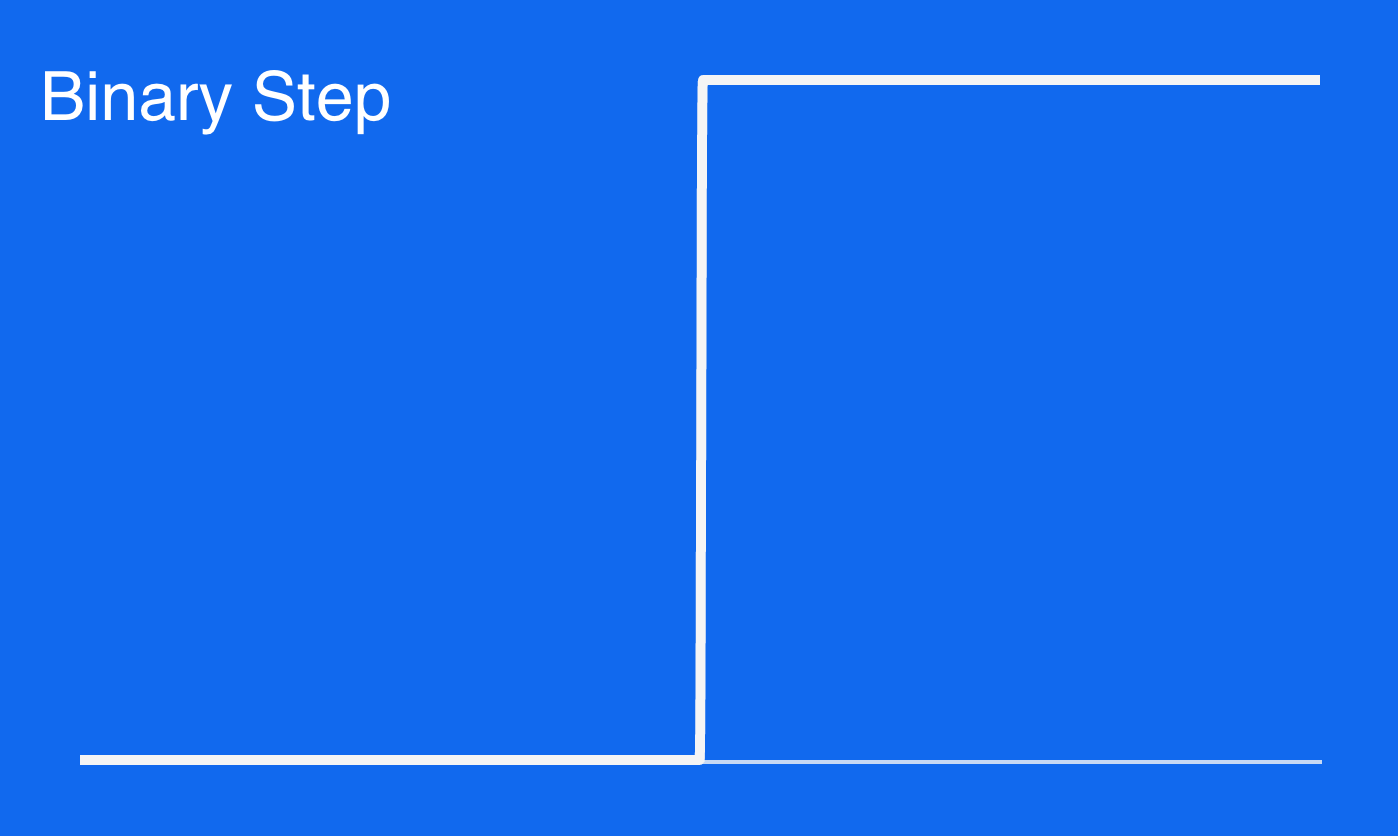
\includegraphics[width=.265\textwidth]{4fig/binary.png}
\caption{Binary Step activation function.}
\end{figure}



\section{Linear}.\\\\

This produces a signal proportional to the input multiplied by each neurons weight. It is an improvement over the step function as it allows for multiple outputs. It does however mean that we are unable to use backpropagation (gradient descent) to train the model. In adition to not being able to improve a model, all the layers in the neural network collapse into a single layer. This means that the final layer will always be a linear function of the first layer. This eliminates all the merits which may be gained from deep learning. A neural network with a linear activation function is simply a linear regression model.

\begin{equation}
    f(x) = m(x)
\end{equation}
\begin{figure}[H]
\centering
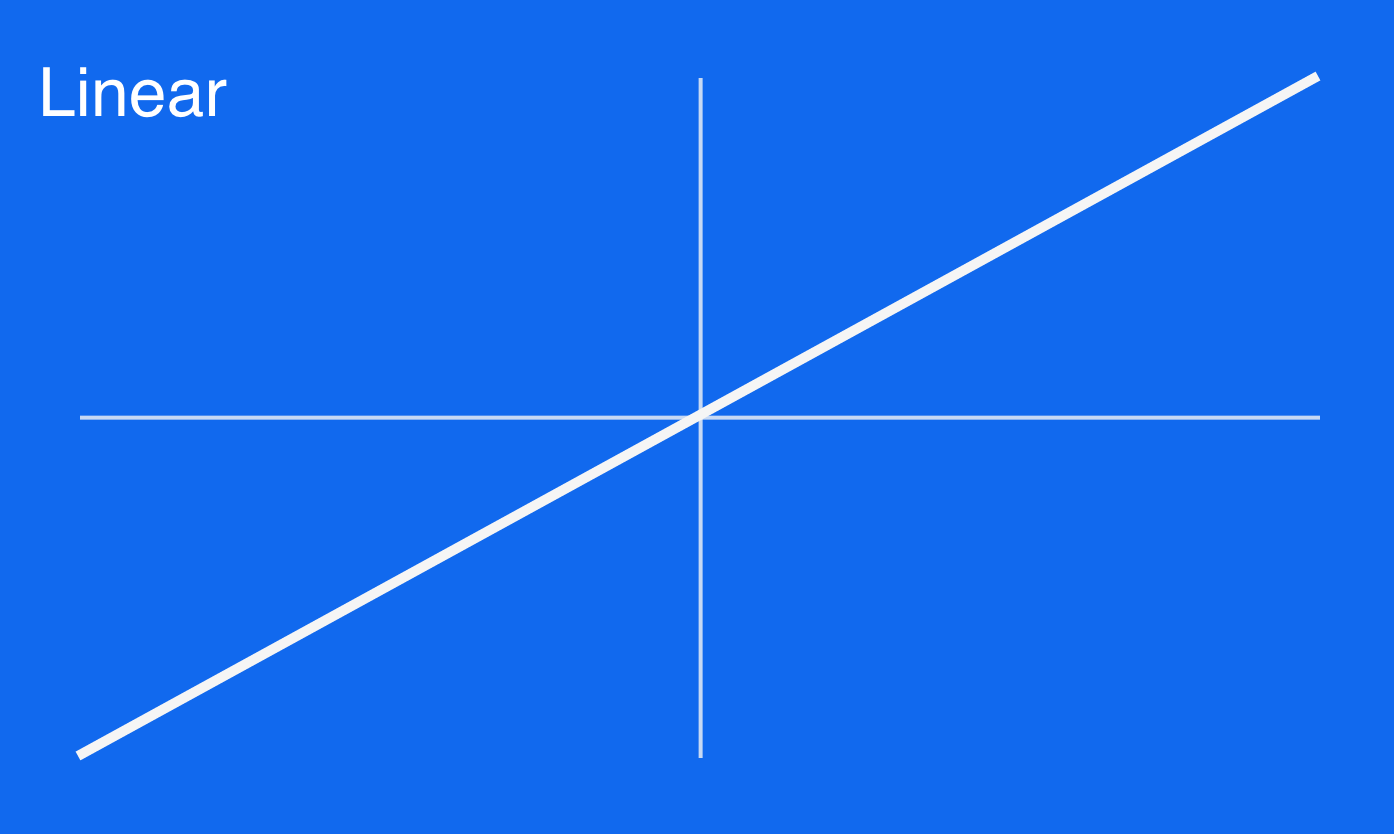
\includegraphics[width=.265\textwidth]{4fig/linear.png}
\caption{Linear activation function.}
\end{figure}

\section{Sigmoid / Logistic}.\\\\
The first of the non-linear activation functions. It has a smooth gradient providing smooth output values which are bound between 1 and 0, normalising the output of each neuron. The main disadvantage is that is falls foul the vanishing gradient problem - for extreme values of $x$ there is close to no change in the prediction. This may result in either early termination of the training, or a slow training cycle in obtaining adequate precision. The activations is computationally expensive and the outputs are not zero centred.

\begin{equation}
    f(x) = 1/1+e^x
\end{equation}
\begin{figure}[H]
\centering
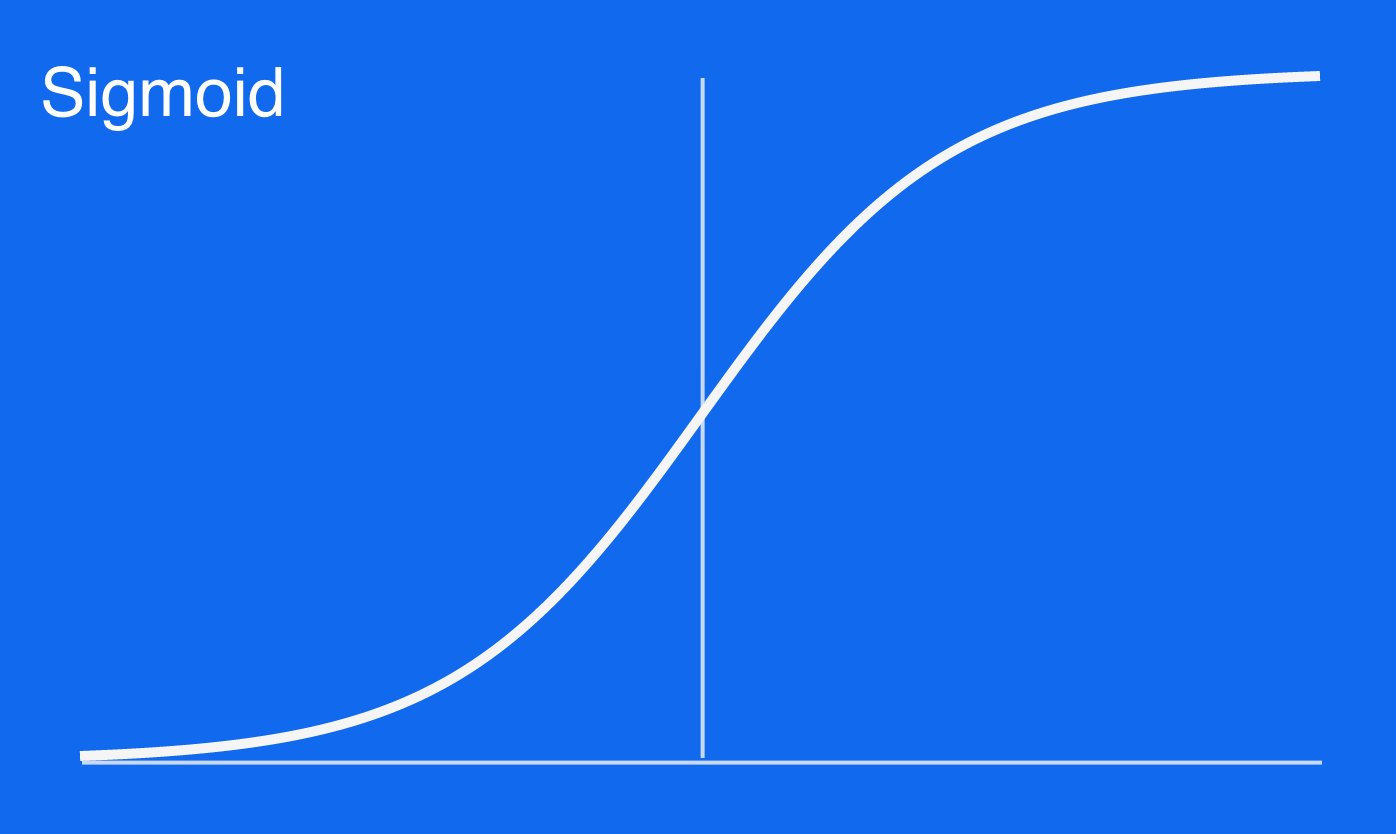
\includegraphics[width=.265\textwidth]{4fig/sigmoid.png}
\caption{Sigmoid activation function.}
\end{figure}


\section{Hyperbolic Tangent}.\\\\
Much like the sigmoid function in both advantages and disadvantages. The hyperbolic tangent function provides a smooth curve which is zero centred. It is however computationally expensive and suffers from the vanishing gradient problem.

\begin{equation}
    f(x) = \frac {e^x - e^{-x}} {e^x + e^{-x}}
\end{equation}
\begin{figure}[H]
\centering
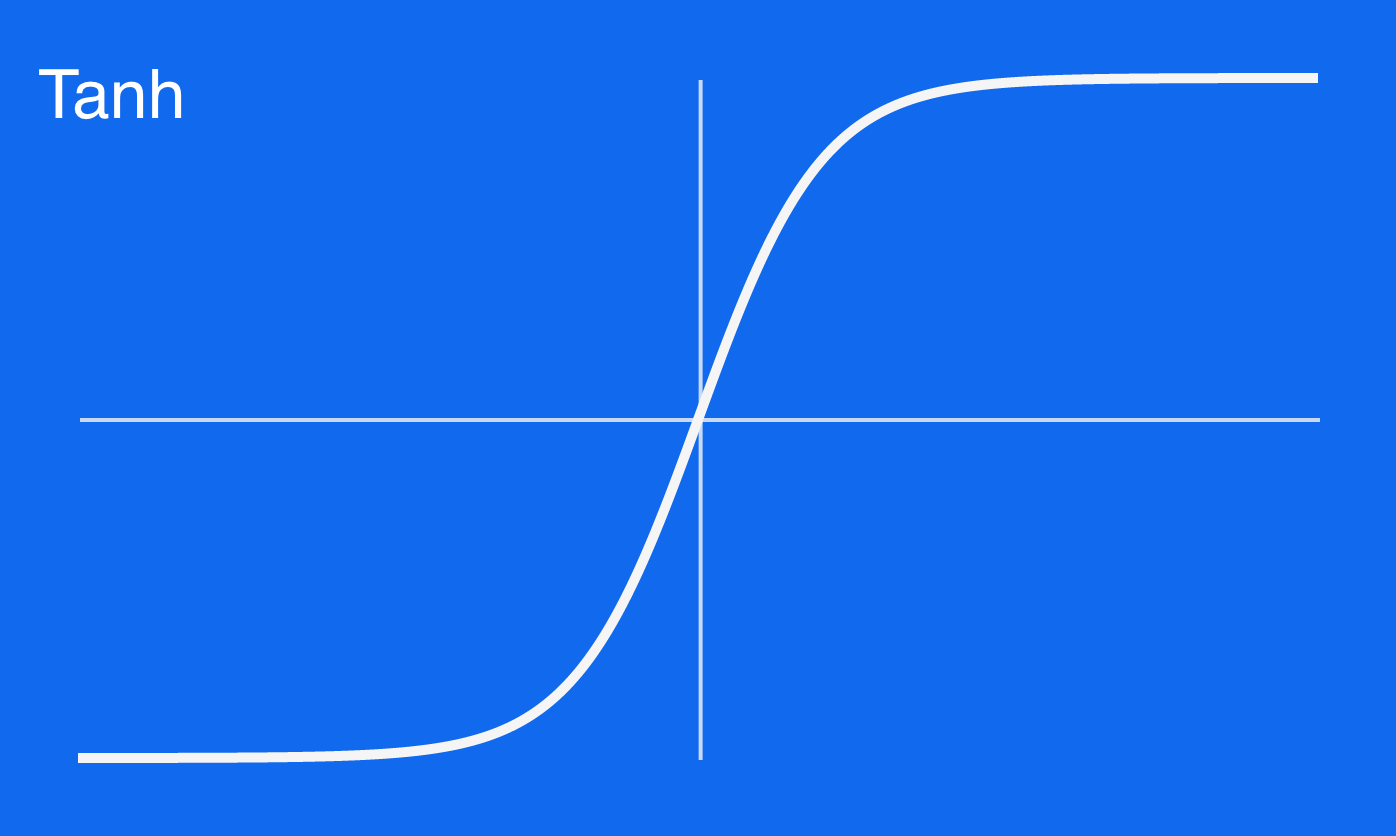
\includegraphics[width=.265\textwidth]{4fig/tanh.png}
\caption{Tanh activation function.}
\end{figure}


\section{Rectified Linear Unit}.\\\\
A commonly used activation for large deep neural networks, due to its computational efficiency and quick convergence. It is non-linear although it appears like a linear function, and allows for back propagation. It does however suffer from the dying ReLU problem - when inputs tend to zero or below, the gradient of the function becomes zero and the network cannot perform backpropagation to learn.

\begin{equation}
f(x) =
    \begin{cases}
      0 , & \mathbf{if} \ x < threshold \\
      x , & \text{otherwise}\\
    \end{cases}
  \end{equation}
\begin{figure}[H]
\centering
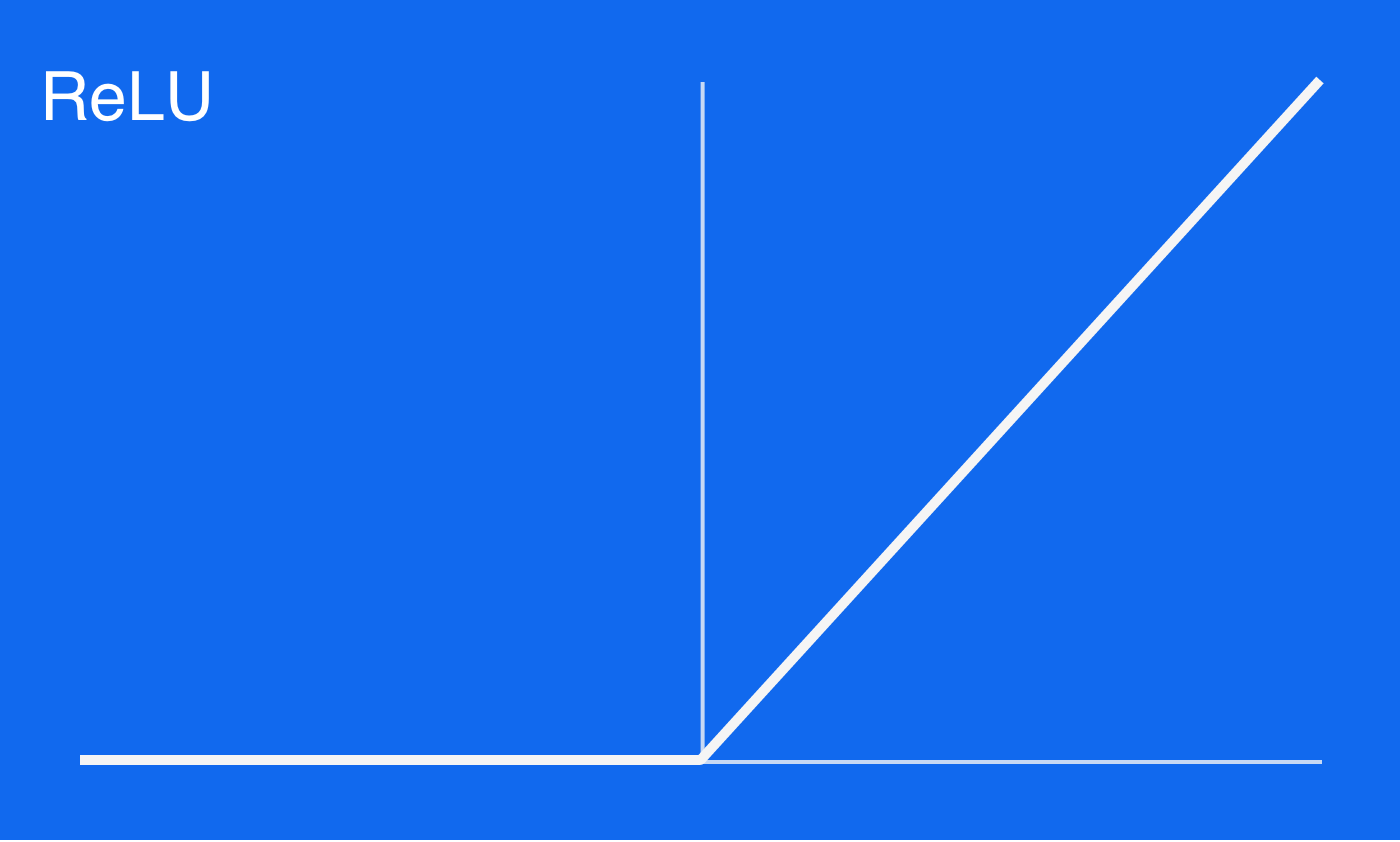
\includegraphics[width=.265\textwidth]{4fig/relu.png}
\caption{ReLU activation function.}
\end{figure}



\section{Swish}.\\\\
https://arxiv.org/abs/1710.05941v1
\textbf{\textit{a new, self-gated activation function discovered by researchers at Google. According to their paper, it performs better than ReLU with a similar level of computational efficiency. In experiments on ImageNet with identical models running ReLU and Swish, the new function achieved top -1 classification accuracy 0.6-0.9\% higher.}}

\begin{equation}
f(x) = x/1-e^{-x}
  \end{equation}
\begin{figure}[H]
\centering
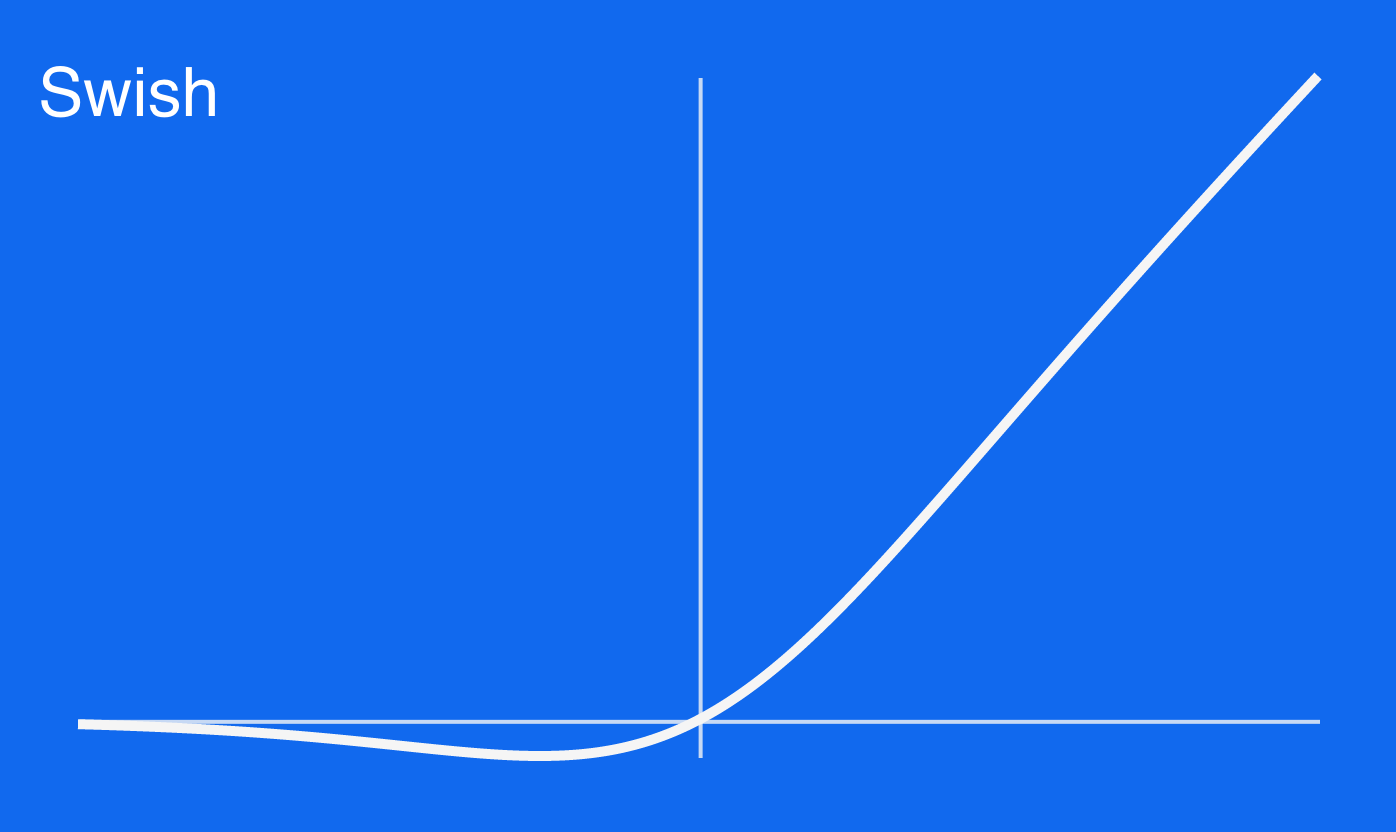
\includegraphics[width=.265\textwidth]{4fig/swish.png}
\caption{Swish activation function.}
\end{figure}

\section{\textbf{A note on backpropagation}}
\emph{As it has not been explicitly explained before back-propagation is an algorithm used to train neural networks. The derivative (or gradient) of an activation function is important in the use of back propagation. Here the model weights are adjusted, and improved, by tracing back all the connections in network, suggesting an optimal weight of each neuron.}


\newpage

\bibliographystyle{apalike} 
\bibliography{ch4,c5ae}
% \bibliographystyle{unsrt}


\newpage
\tableofcontents



\end{document}

